% Options for packages loaded elsewhere
% Options for packages loaded elsewhere
\PassOptionsToPackage{unicode}{hyperref}
\PassOptionsToPackage{hyphens}{url}
%
\documentclass[
  12pt,
  letterpaper,
  openany,
  oneside]{book}
\usepackage{xcolor}
\usepackage[left=2.5cm,right=2.5cm,top=2.5cm,bottom=2.5cm]{geometry}
\usepackage{amsmath,amssymb}
\setcounter{secnumdepth}{5}
\usepackage{iftex}
\ifPDFTeX
  \usepackage[T1]{fontenc}
  \usepackage[utf8]{inputenc}
  \usepackage{textcomp} % provide euro and other symbols
\else % if luatex or xetex
  \usepackage{unicode-math} % this also loads fontspec
  \defaultfontfeatures{Scale=MatchLowercase}
  \defaultfontfeatures[\rmfamily]{Ligatures=TeX,Scale=1}
\fi
\usepackage{lmodern}
\ifPDFTeX\else
  % xetex/luatex font selection
\fi
% Use upquote if available, for straight quotes in verbatim environments
\IfFileExists{upquote.sty}{\usepackage{upquote}}{}
\IfFileExists{microtype.sty}{% use microtype if available
  \usepackage[]{microtype}
  \UseMicrotypeSet[protrusion]{basicmath} % disable protrusion for tt fonts
}{}
\makeatletter
\@ifundefined{KOMAClassName}{% if non-KOMA class
  \IfFileExists{parskip.sty}{%
    \usepackage{parskip}
  }{% else
    \setlength{\parindent}{0pt}
    \setlength{\parskip}{6pt plus 2pt minus 1pt}}
}{% if KOMA class
  \KOMAoptions{parskip=half}}
\makeatother
% Make \paragraph and \subparagraph free-standing
\makeatletter
\ifx\paragraph\undefined\else
  \let\oldparagraph\paragraph
  \renewcommand{\paragraph}{
    \@ifstar
      \xxxParagraphStar
      \xxxParagraphNoStar
  }
  \newcommand{\xxxParagraphStar}[1]{\oldparagraph*{#1}\mbox{}}
  \newcommand{\xxxParagraphNoStar}[1]{\oldparagraph{#1}\mbox{}}
\fi
\ifx\subparagraph\undefined\else
  \let\oldsubparagraph\subparagraph
  \renewcommand{\subparagraph}{
    \@ifstar
      \xxxSubParagraphStar
      \xxxSubParagraphNoStar
  }
  \newcommand{\xxxSubParagraphStar}[1]{\oldsubparagraph*{#1}\mbox{}}
  \newcommand{\xxxSubParagraphNoStar}[1]{\oldsubparagraph{#1}\mbox{}}
\fi
\makeatother


\usepackage{longtable,booktabs,array}
\usepackage{calc} % for calculating minipage widths
% Correct order of tables after \paragraph or \subparagraph
\usepackage{etoolbox}
\makeatletter
\patchcmd\longtable{\par}{\if@noskipsec\mbox{}\fi\par}{}{}
\makeatother
% Allow footnotes in longtable head/foot
\IfFileExists{footnotehyper.sty}{\usepackage{footnotehyper}}{\usepackage{footnote}}
\makesavenoteenv{longtable}
\usepackage{graphicx}
\makeatletter
\newsavebox\pandoc@box
\newcommand*\pandocbounded[1]{% scales image to fit in text height/width
  \sbox\pandoc@box{#1}%
  \Gscale@div\@tempa{\textheight}{\dimexpr\ht\pandoc@box+\dp\pandoc@box\relax}%
  \Gscale@div\@tempb{\linewidth}{\wd\pandoc@box}%
  \ifdim\@tempb\p@<\@tempa\p@\let\@tempa\@tempb\fi% select the smaller of both
  \ifdim\@tempa\p@<\p@\scalebox{\@tempa}{\usebox\pandoc@box}%
  \else\usebox{\pandoc@box}%
  \fi%
}
% Set default figure placement to htbp
\def\fps@figure{htbp}
\makeatother


% definitions for citeproc citations
\NewDocumentCommand\citeproctext{}{}
\NewDocumentCommand\citeproc{mm}{%
  \begingroup\def\citeproctext{#2}\cite{#1}\endgroup}
\makeatletter
 % allow citations to break across lines
 \let\@cite@ofmt\@firstofone
 % avoid brackets around text for \cite:
 \def\@biblabel#1{}
 \def\@cite#1#2{{#1\if@tempswa , #2\fi}}
\makeatother
\newlength{\cslhangindent}
\setlength{\cslhangindent}{1.5em}
\newlength{\csllabelwidth}
\setlength{\csllabelwidth}{3em}
\newenvironment{CSLReferences}[2] % #1 hanging-indent, #2 entry-spacing
 {\begin{list}{}{%
  \setlength{\itemindent}{0pt}
  \setlength{\leftmargin}{0pt}
  \setlength{\parsep}{0pt}
  % turn on hanging indent if param 1 is 1
  \ifodd #1
   \setlength{\leftmargin}{\cslhangindent}
   \setlength{\itemindent}{-1\cslhangindent}
  \fi
  % set entry spacing
  \setlength{\itemsep}{#2\baselineskip}}}
 {\end{list}}
\usepackage{calc}
\newcommand{\CSLBlock}[1]{\hfill\break\parbox[t]{\linewidth}{\strut\ignorespaces#1\strut}}
\newcommand{\CSLLeftMargin}[1]{\parbox[t]{\csllabelwidth}{\strut#1\strut}}
\newcommand{\CSLRightInline}[1]{\parbox[t]{\linewidth - \csllabelwidth}{\strut#1\strut}}
\newcommand{\CSLIndent}[1]{\hspace{\cslhangindent}#1}



\setlength{\emergencystretch}{3em} % prevent overfull lines

\providecommand{\tightlist}{%
  \setlength{\itemsep}{0pt}\setlength{\parskip}{0pt}}



 


\usepackage{booktabs}
\usepackage{caption}
\usepackage{longtable}
\usepackage{colortbl}
\usepackage{array}
\usepackage{anyfontsize}
\usepackage{multirow}
\usepackage{float}
\usepackage{placeins}
\usepackage{fontspec}
\usepackage{xeCJK}
\usepackage{setspace}
\usepackage{titlesec}
\usepackage{placeins}
\setmainfont{texgyreheros-regular.otf}[
  Path = fonts/,
  BoldFont = texgyreheros-bold.otf,
  ItalicFont = texgyreheros-italic.otf,
  BoldItalicFont = texgyreheros-bolditalic.otf
]
\setCJKmainfont{NotoSansCJKtc-Regular.otf}[
  Path = fonts/,
  BoldFont = NotoSansCJKtc-Bold.otf
]
\setstretch{1.5}
\setlength{\parindent}{0pt}
\setlength{\parskip}{6pt}
\titleformat{\chapter}[block]
  {\centering\bfseries\fontsize{18}{27}\selectfont}
  {\chaptername\ \thechapter.}{0.5em}{}
\titlespacing*{\chapter}{0pt}{-20pt}{24pt}
\titleformat{\section}
  {\bfseries\fontsize{14}{21}\selectfont}
  {\thesection}{1em}{}
\titlespacing*{\section}{0pt}{12pt}{6pt}
\titleformat{\subsection}
  {\bfseries\fontsize{12}{18}\selectfont}
  {\thesubsection}{1em}{}
\titlespacing*{\subsection}{0pt}{10pt}{4pt}
\usepackage{caption}
\raggedbottom
\captionsetup[table]{font=bf}
\captionsetup[figure]{labelfont=bf}
\usepackage{etoolbox}
\newif\iffirstsection
\firstsectiontrue
\pretocmd{\chapter}{\firstsectiontrue}{}{}
\pretocmd{\section}{\FloatBarrier\iffirstsection\firstsectionfalse\else\clearpage\fi}{}{}
\pretocmd{\subsection}{\FloatBarrier}{}{}
\AtBeginEnvironment{CSLReferences}{\raggedright}
\renewcommand{\maketitle}{}
\let\realmainmatter\mainmatter
\renewcommand{\mainmatter}{}
\makeatletter
\@ifpackageloaded{bookmark}{}{\usepackage{bookmark}}
\makeatother
\makeatletter
\@ifpackageloaded{caption}{}{\usepackage{caption}}
\AtBeginDocument{%
\ifdefined\contentsname
  \renewcommand*\contentsname{Table of contents}
\else
  \newcommand\contentsname{Table of contents}
\fi
\ifdefined\listfigurename
  \renewcommand*\listfigurename{List of Figures}
\else
  \newcommand\listfigurename{List of Figures}
\fi
\ifdefined\listtablename
  \renewcommand*\listtablename{List of Tables}
\else
  \newcommand\listtablename{List of Tables}
\fi
\ifdefined\figurename
  \renewcommand*\figurename{Figure}
\else
  \newcommand\figurename{Figure}
\fi
\ifdefined\tablename
  \renewcommand*\tablename{Table}
\else
  \newcommand\tablename{Table}
\fi
}
\@ifpackageloaded{float}{}{\usepackage{float}}
\floatstyle{ruled}
\@ifundefined{c@chapter}{\newfloat{codelisting}{h}{lop}}{\newfloat{codelisting}{h}{lop}[chapter]}
\floatname{codelisting}{Listing}
\newcommand*\listoflistings{\listof{codelisting}{List of Listings}}
\makeatother
\makeatletter
\makeatother
\makeatletter
\@ifpackageloaded{caption}{}{\usepackage{caption}}
\@ifpackageloaded{subcaption}{}{\usepackage{subcaption}}
\makeatother
\usepackage{bookmark}
\IfFileExists{xurl.sty}{\usepackage{xurl}}{} % add URL line breaks if available
\urlstyle{same}
\hypersetup{
  pdftitle={My PhD Thesis},
  pdfauthor={Po-Kai Yang},
  hidelinks,
  pdfcreator={LaTeX via pandoc}}


\title{My PhD Thesis}
\author{Po-Kai Yang}
\date{}
\begin{document}
\frontmatter
\maketitle

\thispagestyle{empty}
\begin{center}

{\fontsize{24}{28}\selectfont\bfseries 國立成功大學\par}
\vspace{0.3cm}
{\fontsize{20}{24}\selectfont\bfseries 生物醫學工程系(所)\par}
\vspace{0.3cm}
{\fontsize{20}{24}\selectfont\bfseries 博士學位論文\par}

\vspace{2cm}

{\fontsize{18}{27}\selectfont\bfseries
新式自動化科氏音血壓計於高風險心血管族群之\par
準確度及量測可行性研究\par}

\vspace{1cm}

{\fontsize{16}{24}\selectfont\bfseries
Accuracy and Feasibility of a Novel Automated\par
Korotkoff Sound-Based Blood Pressure Monitor\par
in High-Risk Cardiovascular Patients\par}

\vfill

{\fontsize{16}{24}\selectfont\bfseries 研究生：楊博凱\par}
\vspace{0.4cm}
{\fontsize{16}{24}\selectfont\bfseries 指導教授：葉明龍 教授\par}

\vspace{1.5cm}

{\fontsize{16}{24}\selectfont\bfseries 中華民國一百一十五年五月\par}

\vspace{1cm}

\end{center}
\newpage
\frontmatter
\pagenumbering{roman}
\setcounter{page}{1}


\mainmatter
\bookmarksetup{startatroot}

\chapter*{中文摘要}\label{ux4e2dux6587ux6458ux8981}
\addcontentsline{toc}{chapter}{中文摘要}

\markboth{中文摘要}{中文摘要}

精確的血壓量測對於心血管風險評估及治療決策至關重要。儘管示波法血壓計（Oscillo-BP）已被廣泛使用，但其在高風險心血管族群中的表現可能因心律不整及動脈硬化而受到影響，導致較大的量測誤差與較高的量測失敗率。本研究評估一種新型自動化科氏音血壓計（Ksens-BP），該裝置採用半導體壓阻式微振動感測器擷取動脈壁訊號，並透過深度學習模型自動估算收縮壓與舒張壓，旨在於臨床上具挑戰性的族群中，達到比示波法量測更接近聽診法血壓的一致性。

本研究共納入197位受試者，產生891次量測嘗試。排除非儀器相關之嘗試（人為操作疏失，n
= 3；嚴重顫抖，n =
4）後，884次嘗試納入可行性評估。Oscillo-BP於884次嘗試中有143次量測失敗（16.2\%），而Ksens-BP之擷取錯誤為61次（6.9\%），其中包含6次兩系統同時失敗。最終，來自178位受試者的686次成功量測納入一致性分析。以聽診法血壓作為參考標準，Ksens-BP在收縮壓與舒張壓之一致性相關係數均優於Oscillo-BP，且兩個壓力域之平均絕對誤差均顯著較小。Oscillo-BP呈現系統性舒張壓低估，此現象與固定比率示波法演算法對動脈硬化之已知敏感性一致------此偏差在Ksens-BP系統中未被觀察到。混合效應模型分析顯示，男性為Oscillo-BP收縮壓差異較大之獨立預測因子，而Ksens-BP則無相應影響。心房顫動為示波法量測失敗之主要預測因子，在嘗試層級之調整勝算比超過13，而科氏音偵測則不受心律不規則之影響，仍可正常運作。

在此富含動脈粥狀硬化共病之心血管門診族群中，Ksens-BP所提供之血壓估計值與聽診法量測結果的一致性顯著優於Oscillo-BP，尤其在舒張壓一致性、不受性別影響之量測穩定性，以及心房顫動患者之量測可行性方面具有明顯優勢。上述發現顯示，K-Sensor方法在示波法量測模型結構性受限之患者族群中，可作為一種技術上與臨床上均具獨特性之替代方案。

\textbf{關鍵詞：}
血壓量測、科氏音、示波法血壓計、心房顫動、動脈硬化、自動化血壓計

\bookmarksetup{startatroot}

\chapter*{Abstract}\label{abstract}
\addcontentsline{toc}{chapter}{Abstract}

\markboth{Abstract}{Abstract}

Accurate blood pressure (BP) measurement is crucial for cardiovascular
risk assessment and therapeutic decision-making. Although oscillometric
BP monitors (Oscillo-BP) are widely used, their performance in high-risk
cardiovascular populations may be compromised by arrhythmia and arterial
stiffness, resulting in larger measurement discrepancies and higher
failure rates. This study evaluated a novel automated Korotkoff
sound-based BP monitor (Ksens-BP) that uses a semiconductor
piezoresistive microvibration sensor to capture arterial wall signals
and a deep-learning model to automatically estimate systolic and
diastolic BP, aiming to achieve closer agreement with auscultatory BP
than oscillometric measurement in clinically challenging cohorts.

A total of 197 participants were enrolled from a cardiovascular
outpatient center, yielding 891 attempted measurements. After excluding
non-device-related attempts (human operation error, n = 3; severe
tremor, n = 4), 884 attempts were eligible for feasibility evaluation.
Oscillo-BP failed in 143/884 attempts (16.2\%), whereas Ksens-BP
acquisition errors occurred in 61/884 attempts (6.9\%), including 6
attempts with concurrent failures of both systems. Ultimately, 686
successful measurements from 178 participants were included in the
agreement analysis. Using auscultatory BP as the reference standard,
Ksens-BP demonstrated stronger agreement than Oscillo-BP, with higher
concordance correlation coefficients for both systolic and diastolic BP.
Ksens-BP achieved significantly smaller mean absolute errors for both
pressure domains compared with Oscillo-BP. Oscillo-BP exhibited a
systematic diastolic underestimation consistent with the known
sensitivity of fixed-ratio oscillometric algorithms to arterial
stiffness - a bias absent in the Ksens-BP system. Mixed-effects modeling
identified male sex as an independent predictor of larger Oscillo-BP
systolic discrepancy, with no corresponding effect on Ksens-BP. Atrial
fibrillation was the dominant predictor of oscillometric measurement
failure, with an adjusted odds ratio exceeding 13 at the attempt level,
whereas K-sound-based detection remained viable regardless of cardiac
rhythm irregularity.

In this cardiovascular outpatient cohort enriched with atherosclerotic
comorbidities, Ksens-BP provided BP estimates with substantially closer
agreement with auscultatory measurements than Oscillo-BP, with
particular advantages in diastolic agreement, sex-independent
measurement consistency, and measurement feasibility in atrial
fibrillation. These findings position the K-Sensor approach as a
technically and clinically distinct alternative to oscillometry for
patient populations in whom the oscillometric measurement model is
structurally compromised.

\textbf{Keywords:} blood pressure measurement; Korotkoff sounds;
oscillometric blood pressure monitor; atrial fibrillation; arterial
stiffness; automated blood pressure device

\cleardoublepage
\phantomsection
\addcontentsline{toc}{chapter}{Table of Contents}
\tableofcontents
\cleardoublepage

\phantomsection
\addcontentsline{toc}{chapter}{List of Figures}
\listoffigures
\cleardoublepage

\phantomsection
\addcontentsline{toc}{chapter}{List of Tables}
\listoftables
\cleardoublepage

\realmainmatter
\pagenumbering{arabic}
\setcounter{page}{1}

\bookmarksetup{startatroot}

\chapter{Introduction}\label{introduction}

\section{Background}\label{background}

Accurate BP measurement remains a cornerstone in the diagnosis of
hypertension, the evaluation of cardiovascular risk, and the management
of therapeutic strategies. Although measurement technologies have
advanced significantly over the past decades, the pursuit of a method
that is universally accurate, reliable, and feasible in various clinical
settings is still ongoing. For more than a century, the auscultatory
method using a mercury sphygmomanometer has been recognized as the gold
standard for non-invasive blood pressure (BP) measurement in clinical
settings\textsuperscript{1}. This method entails the inflation of an arm
cuff to occlude arterial blood flow-most commonly in the brachial
artery-followed by gradual deflation while a trained observer detects
Korotkoff sounds(K-sounds) via stethoscope(Figure 1.1). The onset of the
first K-sound (phase I) is interpreted as the systolic blood pressure
(SBP), whereas the disappearance of the sounds (phase V) typically marks
the diastolic blood pressure
(DBP)(Table~\ref{tbl-ksound-phases})\textsuperscript{2}. The K-sounds
are characterized by five distinct phases: Phase I (clear tapping),
Phase II (swooshing sounds or murmurs), Phase III (crisper, more intense
tapping), Phase IV (abrupt muffling of sounds), and Phase V (silence, or
the disappearance of sounds). Accurate identification of these phases,
particularly I and V (or IV in certain populations), is paramount for
correct BP assessment. The durability, straightforward design, and high
inter-device consistency of mercury sphygmomanometers across
manufacturers have all contributed to their longstanding acceptance and
reliability in clinical practice. Manual blood pressure measurement
using K-sound is subject to several limitations, primarily related to
human error and observer variability\textsuperscript{2}. Inaccurate cuff
or stethoscope placement, difficulty detecting faint sounds due to noise
or inattention, and inconsistencies in identifying the precise pressure
at which sounds appear or disappear can all compromise accuracy. Studies
have shown that even small changes in stethoscope positioning can lead
to significant variations in readings\textsuperscript{3}. Inter-observer
variability further reduces reliability, as differences in technique,
experience, and hearing acuity can result in inconsistent measurements
from the same patient. Environmental factors also affect measurement
quality. Background noise, common in clinical settings, can obscure
K-sounds, especially the softer Phase I and V sounds. In addition, while
often considered straightforward, manual BP measurement requires careful
technique and proper training. It is time-consuming and may not be
practical in high-volume or emergency care settings, where speed and
consistency are critical. Despite these challenges, the mercury
sphygmomanometer remains particularly valuable when clinical decisions
are based on precise blood pressure readings, as the method provides
unparalleled accuracy when performed correctly.

\begin{figure}[H]

{\centering \pandocbounded{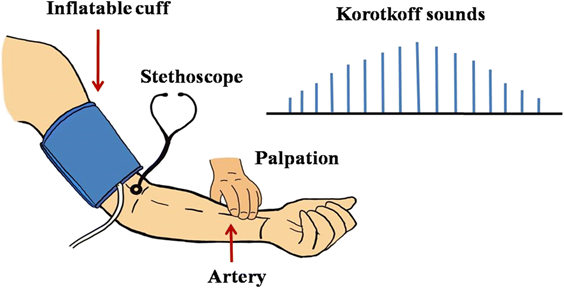
\includegraphics[keepaspectratio]{chapters/../outputs/figures/External/1-1.png}}

}

\caption[BP measurement by auscultatory
method.]{\textbf{BP measurement by auscultatory method.} An inflatable
upper-arm cuff is inflated to occlude the brachial artery and then
slowly deflated while Korotkoff sounds are detected with a stethoscope
placed over the artery. The appearance of the first Korotkoff sound
during deflation indicates systolic blood pressure, and the
disappearance of Korotkoff sounds indicates diastolic blood pressure.}

\end{figure}%

\begin{longtable}[]{@{}
  >{\raggedright\arraybackslash}p{(\linewidth - 2\tabcolsep) * \real{0.5000}}
  >{\raggedright\arraybackslash}p{(\linewidth - 2\tabcolsep) * \real{0.5000}}@{}}
\caption{Korotkoff Sound Phases}\label{tbl-ksound-phases}\tabularnewline
\toprule\noalign{}
\begin{minipage}[b]{\linewidth}\raggedright
Phase
\end{minipage} & \begin{minipage}[b]{\linewidth}\raggedright
Qualitative description
\end{minipage} \\
\midrule\noalign{}
\endfirsthead
\toprule\noalign{}
\begin{minipage}[b]{\linewidth}\raggedright
Phase
\end{minipage} & \begin{minipage}[b]{\linewidth}\raggedright
Qualitative description
\end{minipage} \\
\midrule\noalign{}
\endhead
\bottomrule\noalign{}
\endlastfoot
I & Appearance: The first loud tapping sound heard; systolic pressure \\
II & Softening: Weakened clapping sound and soft wind-like murmur \\
III & Sharpening: Blowing wind-like murmur disappears \\
IV & Muffling: The tone is suddenly dull \\
V & Disappearance: Loss of sound; diastolic pressure \\
\end{longtable}

\section{Oscillometric Method Principles and
Limitations}\label{oscillometric-method-principles-and-limitations}

\subsection{Fundamental mechanisms}\label{fundamental-mechanisms}

The inherent limitations and practical inconveniences of auscultatory
blood pressure measurement have naturally led to the emergence of
automated blood pressure monitoring technologies. Among these,
oscillometric devices have become the most widely used form of automated
blood pressure monitors in clinical and home settings. The widespread
adoption of automated oscillometric blood pressure monitors has
fundamentally transformed clinical practice, offering convenience,
standardization, and reduced dependence on operator
skill\textsuperscript{4}. Similar to the auscultatory method, the
oscillometric technique also requires the use of an inflatable cuff
placed on the upper arm to occlude arterial blood flow. As the cuff
gradually deflates and the pressure falls below the SBP, blood flow
resumes intermittently. These intermittent flows cause the arterial wall
beneath the cuff to expand and contract with each cardiac cycle. The
resulting arterial wall movements generate pulsations that are
transmitted to the air within the cuff, producing small, superimposed
pressure oscillations. These oscillations serve as the primary signal
detected by the device's internal pressure sensor, which typically
consists of a piezoresistive silicon transducer\textsuperscript{5}.

The sensor detects raw signals composed of gradually declining cuff
pressure overlaid with small pressure oscillations generated by arterial
pulsations. These signals undergo filtering to remove low-frequency
baseline drift and high-frequency noise, followed by amplification to
enhance the oscillometric waveform (OMW). From the processed OMW, an
oscillometric pulse index (OPI) is calculated for each cardiac
cycle-commonly defined by parameters such as peak-to-peak amplitude or
area under the pulse. Plotting OPI values against corresponding cuff
pressures yields the oscillometric waveform envelope
(OMWE)\textsuperscript{6}, which is often smoothed using curve-fitting
methods. A key principle in this approach is the Maximum Amplitude
Algorithm, which identifies the cuff pressure at the peak of the OMWE as
the mean arterial pressure (MAP)\textsuperscript{6}. This peak
corresponds to the point where cuff pressure equals intra-arterial
pressure, resulting in maximal arterial wall oscillation. As such, MAP
is generally regarded as the most accurate parameter derived from
oscillometric measurements.

Unlike MAP, SBP and DBP are not directly identified by a unique,
universally agreed-upon feature of the OMWE. Instead, they are estimated
or calculated based on the characteristics of the OMWE, often in
relation to the already determined MAP, using proprietary algorithms
that vary between device manufacturers\textsuperscript{4}.

\begin{figure}[H]

{\centering \pandocbounded{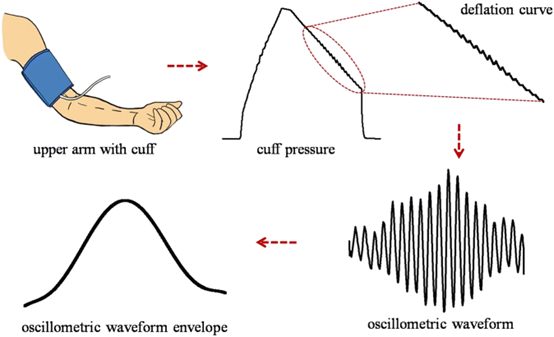
\includegraphics[keepaspectratio]{chapters/../outputs/figures/External/1-2.png}}

}

\caption[BP measurement of oscillometric
method.]{\textbf{BP measurement of oscillometric method.} An upper-arm
cuff is inflated above arterial occlusion pressure and then gradually
deflated. During deflation, arterial volume changes induce pressure
oscillations that are superimposed on the cuff pressure signal
(oscillometric waveform). The oscillation amplitude increases as cuff
pressure approaches MAP and then decreases. SBP and DBP are estimated
from the envelope using device-specific algorithms.}

\end{figure}%

\subsection{Systematic Limitations and Accuracy
Concerns}\label{systematic-limitations-and-accuracy-concerns}

The oscillometric method operates on the principle of detecting pressure
oscillations within the arterial wall during controlled cuff deflation,
utilizing maximum amplitude algorithms to determine blood pressure
values\textsuperscript{4}. Unlike auscultatory methods that rely on
auditory detection of K-sounds, oscillometric devices measure the
amplitude of pressure oscillations transmitted through the arterial wall
to the cuff\textsuperscript{7}. The algorithm identifies the cuff
pressure corresponding to maximum oscillation amplitude as the mean
arterial pressure, while SBP and DBP are calculated using predetermined
ratios. This automated approach eliminates observer variability and
provides consistent measurement protocols, making it particularly
attractive for standardized clinical applications. However, the reliance
on algorithmic interpretation of pressure oscillations introduces
specific limitations that affect measurement accuracy in patients with
altered vascular mechanics\textsuperscript{7}. These algorithms, which
dictate how MAP is precisely identified and how SBP and DBP are
subsequently derived from the OMWE, are typically considered trade
secrets by manufacturers and are not publicly disclosed for independent
critique or validation. This lack of transparency, often referred to as
the ``black box'' issue, presents several critical challenges. It
prevents a clear understanding of why different devices may yield
inconsistent readings for the same patient, complicates efforts to
assess the impact of specific physiological conditions such as increased
arterial stiffness or atrial fibrillation, and obstructs the development
of standardized correction methods to improve measurement reliability
across diverse populations and devices. Moreover, because these
algorithms are often developed using data from individuals with presumed
normal cardiovascular profiles, their accuracy may be compromised in
patients with abnormal hemodynamics. As a result, the reliance on
algorithmic inference rather than direct physiological measurement
remains a fundamental source of error and uncertainty.

In a study of 337 cardiology outpatients, BP was measured simultaneously
using both a mercury manometer and an automated oscillometric device.
Mercury readings were significantly higher than oscillometric values for
both systolic and diastolic pressures (p \textless{} 0.0001), with
discrepancies seen in over 20\% of patients. The average differences
were 1.95 mmHg (systolic) and 1.3 mmHg (diastolic), with greater
discrepancies observed in patients over 65\textsuperscript{8}. A
meta-analysis comparing oscillometric readings to invasive arterial
pressure found that while mean arterial pressure showed a small average
bias of -1.50 mmHg, the limits of agreement were wide (from -14.6 mmHg
to +40.3 mmHg)\textsuperscript{9}. Such variability reduces the
reliability of oscillometric methods in clinical situations where
precise blood pressure control is essential.

\subsection{Issues in Atherosclerotic Cardiovascular
Disease}\label{issues-in-atherosclerotic-cardiovascular-disease}

Atherosclerotic cardiovascular disease (ASCVD) significantly alters
arterial wall mechanics, thereby compromising the accuracy of
oscillometric blood pressure (BP) measurements. Arterial stiffening, a
hallmark of ASCVD, results primarily from wall thickening and elastin
degeneration-each contributing differently to measurement error. As
arterial stiffness increases, the characteristics of the arterial
pressure wave are altered, subsequently affecting the amplitude and
shape of cuff pressure oscillations\textsuperscript{10}. In individuals
with compliant arteries, the peak of the OMWE is typically well-defined
and narrow. However, in older adults or patients with stiffened
arteries-conditions often accompanied by a widened pulse pressure-the
OMWE peak becomes broader and flatter. Since SBP and DBP are derived
algorithmically from the OMWE in reference to the identified MAP, such
morphological changes in the envelope inevitably introduce inaccuracies
in the estimation of SBP and DBP\textsuperscript{11}. Wall thickening is
associated with overestimation of SBP, whereas elastin degeneration
affects both SBP and DBP\textsuperscript{7,12}. In advanced stages of
ASCVD, especially among patients with diabetes or end-stage renal
disease, extensive arterial calcification further complicates
measurement. Calcified vessels become rigid and poorly compressible,
limiting the cuff's ability to fully occlude the artery or detect
oscillometric signals accurately, thus exacerbating measurement
inaccuracy\textsuperscript{13}. Insights from computational modeling
have elucidated that such structural changes in the arterial wall
markedly affect pressure transmission dynamics during cuff inflation and
deflation, thereby compromising the reliability of oscillometric
readings\textsuperscript{7}. These findings are consistent with clinical
observations of pseudo-hypertension in elderly individuals with advanced
atherosclerosis, where heightened arterial stiffness requires greater
external cuff pressure to achieve arterial occlusion, thereby leading to
falsely elevated blood pressure measurements. The clinical implications
of these inaccuracies are substantial, as they may lead to overdiagnosis
of hypertension and unwarranted therapeutic interventions. A simulation
study\textsuperscript{14} further supports these concerns by
demonstrating that arterial stiffening-characterized by changes in the
symmetry and steepness of the artery-cuff pressure/volume
relationship-can induce substantial errors in oscillometric BP
estimation. Their findings showed that SBP errors could reach up to
+11.6 mmHg, while diastolic errors varied from over- to underestimation
depending on the combination of arterial compliance parameters. Notably,
mean arterial pressure errors were the most variable, with deviations as
large as ±17.5 mmHg. These errors were strongly influenced by pulse
pressure and the mismatch between the arterial pulse shape index and the
cuff pressure/volume symmetry index, emphasizing the complexity and
vulnerability of oscillometric estimation algorithms in the presence of
altered arterial mechanics. The impact of atherosclerosis on
oscillometric accuracy extends beyond individual variability and carries
implications for broader patient populations. Evidence from studies
investigating arterial stiffness indices suggests that conventional
compliance assessments under physiologic pressure ranges may be
insufficient to predict oscillometric accuracy in patients with marked
vascular pathology. Accordingly, there is an urgent need to develop
alternative BP assessment modalities or calibration strategies in
populations with elevated cardiovascular risk and structural vascular
abnormalities.

\subsection{Specific Problems in Atrial Fibrillation
Patients}\label{specific-problems-in-atrial-fibrillation-patients}

Atrial fibrillation (AF) presents unique challenges for oscillometric BP
measurement due to the inherent irregularity of cardiac rhythm and
stroke volume variation\textsuperscript{15}. The hallmark of AF is a
chaotic and irregular atrial activity, resulting in an irregularly
irregular ventricular response. This irregularity in ventricular
contractions leads to marked beat-to-beat variations in ventricular
filling time and stroke volume. Consequently, there is substantial
beat-to-beat variability in both SBP and DBP. Studies quantifying this
variability have shown that, compared to individuals in sinus rhythm,
patients with AF exhibit approximately a doubling of SBP variability and
a six-fold increase in diastolic BP variability\textsuperscript{16}. The
oscillometric method relies on consistent pressure oscillations for
accurate algorithmic interpretation, but AF introduces significant
beat-to-beat variability that can confound measurement
accuracy\textsuperscript{17}. The accuracy of oscillometric BP
measurement in AF is not uniform across all devices. Significant
discrepancies exist among different validation studies. Pagonas et
al.\textsuperscript{18} studied the Omron M5 Professional (upper arm)
and R5 Professional (wrist) devices against invasive arterial pressure.
They concluded that if three consecutive measurements were averaged, AF
did not significantly affect the mean bias of SBP and DBP. However, they
did find that the within-subject variability of oscillometric
measurements was significantly higher in patients with AF compared to
those in sinus rhythm. Another study\textsuperscript{19} using the
Microlife BP A6 PC (which has an AF detection system) found that,
compared to the auscultatory method, the device reported SBP values that
were on average 5.3 mmHg higher in sinus rhythm patients and 6.1 mmHg
higher in AF patients. While the mean differences were relatively small,
the limits of agreement were very wide ( -23.9 to 11.7 mmHg for SBP in
AF), indicating poor individual reliability. Feenstra et
al.\textsuperscript{17} compared two oscillometric devices-the Welch
Allyn Spot Vital Signs (WASVS) and Philips M3002A IntelliVue X2-against
the Volume Clamp Method in patients with AF. The WASVS showed deviations
of +0.1±14.8mmHg for SBP and +6.3±9.2mmHg for DBP, while the Philips
device showed 6.8±13.2mmHg for SBP and +9.4±8.1mmHg for DBP. Notably,
high beat-to-beat variability and elevated heart rate reduced the
accuracy of the WASVS. The study concluded that oscillometric BP
measurement in AF is generally limited in accuracy and may be unreliable
in individual cases. Accordingly, oscillometric BP values obtained in AF
should be interpreted as estimates whose accuracy depends on the
specific device and the measurement conditions; clinicians should
therefore interpret these readings with caution rather than treating
them as interchangeable physiologic truth.

Table~\ref{tbl-sphygmo-comparison} presents a comparison of the
strengths and limitations of the two blood pressure measurement methods.

\begin{longtable}[]{@{}
  >{\raggedright\arraybackslash}p{(\linewidth - 6\tabcolsep) * \real{0.2500}}
  >{\raggedright\arraybackslash}p{(\linewidth - 6\tabcolsep) * \real{0.2500}}
  >{\raggedright\arraybackslash}p{(\linewidth - 6\tabcolsep) * \real{0.2500}}
  >{\raggedright\arraybackslash}p{(\linewidth - 6\tabcolsep) * \real{0.2500}}@{}}
\caption{Comparative overview of Sphygmomanometer
Technologies}\label{tbl-sphygmo-comparison}\tabularnewline
\toprule\noalign{}
\begin{minipage}[b]{\linewidth}\raggedright
Type
\end{minipage} & \begin{minipage}[b]{\linewidth}\raggedright
Advantages
\end{minipage} & \begin{minipage}[b]{\linewidth}\raggedright
Limitations
\end{minipage} & \begin{minipage}[b]{\linewidth}\raggedright
Validation status
\end{minipage} \\
\midrule\noalign{}
\endfirsthead
\toprule\noalign{}
\begin{minipage}[b]{\linewidth}\raggedright
Type
\end{minipage} & \begin{minipage}[b]{\linewidth}\raggedright
Advantages
\end{minipage} & \begin{minipage}[b]{\linewidth}\raggedright
Limitations
\end{minipage} & \begin{minipage}[b]{\linewidth}\raggedright
Validation status
\end{minipage} \\
\midrule\noalign{}
\endhead
\bottomrule\noalign{}
\endlastfoot
Manual auscultatory & Gold standard; simple design; consistent across
manufacturers. & Environmental toxicity of mercury leading to phase-out;
requires trained observer; susceptible to observer bias. &
Well-established \\
Automated oscillometric & Automated; no observer needed for reading;
less susceptible to external noise. & Indirect estimation of SBP/DBP;
proprietary algorithms vary and are often unpublished; accuracy issues
in specific populations (AF, arterial stiffness, shock). & Calibration
against auscultatory sphygmomanometry is required \\
\end{longtable}

\section{Development Status of Automated K-sound
Devices}\label{development-status-of-automated-k-sound-devices}

Given the respective advantages and limitations of the auscultatory and
oscillometric blood pressure measurement methods, considerable research
efforts have been directed toward developing more advanced and automated
approaches. Among these, automated K-sound detection technology has
emerged as a promising solution to meet this clinical need. The
automation of K-sound detection addresses several critical clinical
needs simultaneously. First, it preserves the physiological accuracy of
the auscultatory method while eliminating the requirement for
specialized operator training\textsuperscript{20}. Second, automated
systems can provide consistent, reproducible measurements that are not
subject to human perception variability or
fatigue\textsuperscript{21,22}. Third, these systems can incorporate
advanced signal processing techniques to enhance detection of weak or
masked K-sounds that might be missed by human
observers\textsuperscript{23}. Moreover, it provides direct
physiological measurements of BP, thereby offering improved fidelity and
reliability, particularly under challenging clinical
conditions\textsuperscript{24}.

The quest for more reliable and objective BP measurement has driven
extensive research and development of automated devices based on
K-sounds. This effort includes advancements in sensor technologies, and
the development of refined algorithms for detecting and interpreting
these sounds

\subsection{Sensor technology and K-sound
Acquisition}\label{sensor-technology-and-k-sound-acquisition}

The accurate capture of K-sounds is the foundational step for any
automated auscultatory system. To achieve this, researchers have
investigated various sensor modalities, evolving from adaptations of
conventional acoustic instruments to the use of novel materials and
innovative designs. Many automated K-sound systems utilize miniature
microphones or electronic stethoscopes integrated within or adjacent to
the BP cuff\textsuperscript{24}. These sensors aim to replicate the
function of a clinician's stethoscope by converting the acoustic energy
of K-sounds into electrical signals. For example, Pan et
al.\textsuperscript{25} utilized two electronic stethoscopes-one
positioned under the cuff and another outside of it-to collect K-sound
data for a deep learning model. Commercially available devices such as
the InBody BPBIO480KV and the KOROT V2 Doctor integrate electronic
stethoscopes within the cuff assembly and often provide clinicians with
features like audible playback or visual display of detected
sounds\textsuperscript{20,26}. Despite their practicality,
microphone-based systems are often sensitive to ambient noise and
require careful acoustic coupling to the skin to ensure signal quality.

Polyvinylidene Fluoride(PVDF) is a flexible, biocompatible piezoelectric
polymer that has been effectively utilized as a contact microphone for
K-sound acquisition. Xiong et al.\textsuperscript{27} developed a device
featuring a 1.4 × 1.4 cm PVDF film sensor with a capacitance of 700 pF,
which was mounted over the brachial artery. The flexibility of PVDF
allows for good conformity to the arm's curvature, potentially improving
signal acquisition. Research has also explored alternative piezoelectric
materials, such as lead zirconate titanate (PZT) ceramics and novel
flexible piezoelectrets\textsuperscript{28}. PZT offers high
piezoelectric coefficients but is inherently rigid. In contrast,
flexible piezoelectrets-consist of charged polymer films with internal
air cavities, allowing them to exhibit piezoelectric
behavior\textsuperscript{29}. These materials can be fabricated into
thin, flexible patches suited for wearable applications. Notably, they
have demonstrated high sensitivity and strong electromagnetic
interference (EMI) shielding in detecting a variety of physiological
sounds, including K-sounds.

\subsection{Algorithmic Approaches to K-Sound Detection and
Interpretation}\label{algorithmic-approaches-to-k-sound-detection-and-interpretation}

Essential preliminary steps in K-sound analysis involve filtering and
amplification. Filtering is crucial for isolating the K-sound signals,
which typically lie in a frequency range of 20-300 Hz or 20-400 Hz, from
background noise and other irrelevant
frequencies\textsuperscript{23,30,31}. The filtered signal is then often
amplified to ensure its amplitude is adequate for processing by
microcontrollers or for further detailed analysis. After signal
processing, several algorithms have been developed to detect K-sound
events associated with SBP and DBP: Threshold-Based Detection: This is
one of the more direct approaches, aiming to mimic the human auditory
detection process. SBP is typically identified as the cuff pressure at
which K-sounds of sufficient amplitude first appear, and DBP as the
pressure at which these sounds disappear or fall below a pre-defined
threshold. In some implementations, the threshold is empirically
determined based on averaged values from manual
measurements\textsuperscript{30}. Power-Based Detection: This method
analyzes the signal energy or power of the K-sound signal, typically in
the frequency domain, during each pulse cycle. SBP is identified at the
point of a marked increase in signal power, while DBP corresponds to a
substantial decrease in power between successive pulses, indicating the
end of audible K-sounds\textsuperscript{30}. Morphological Analysis:
Some algorithms focus on the shape (morphology) of the K-sound
waveforms. The B3X algorithm, for instance, evaluates the beat-by-beat
changes in the morphology of adjacent K-sound pulses by calculating
their cross-correlation\textsuperscript{32}. Significant changes in
waveform shape can indicate the onset or cessation of true K-sounds.
Time-Frequency Analysis: Techniques such as the short-time Fourier
transform (STFT) and wavelet transform are used to capture temporal
changes in the frequency content of K-sound signals. Features derived
from these analyses can improve the accuracy of phase
identification\textsuperscript{30}. Deep Learning for K-Sound Analysis:
The integration of Artificial Intelligence techniques into the analysis
of K-sound represents a significant step in the evolution of automated
BP monitoring. Deep learning techniques, especially Convolutional Neural
Networks (CNNs) and Recurrent Neural Networks (RNNs), have been
increasingly applied to automate the analysis of K sounds. These models
are capable of learning complex temporal and spectral patterns directly
from raw or minimally processed signals. CNNs are commonly used for
classifying audio segments as containing K-sounds or not, as well as for
extracting relevant features. Input data often take the form of
spectrograms or band-pass filtered signal stacks, with the latter
offering better frequency resolution and phase preservation for
short-duration, low-frequency K-sounds\textsuperscript{24}. CNN
architectures typically consist of multiple convolutional and pooling
layers; for instance, Pan et al.\textsuperscript{25} used a 3-layer CNN,
while Chang et al.\textsuperscript{24} adapted ResNet-18. Training
relies on labeled data, either from expert annotation or
probability-based methods. The outputs-K-sound presence probabilities or
classifications-are then mapped to SBP and DBP using predefined decision
rules, such as identifying the first and last appearance of classified
beats or minimizing error against idealized probability curves. RNNs,
particularly Long Short-Term Memory (LSTM) networks, are well-suited for
sequential K-sound data. They can model temporal dependencies across
beats, making them potentially more robust in handling cases like the
auscultatory gap. LSTMs can incorporate contextual patterns over time,
which may improve the detection of SBP and DBP under noisy or
non-standard conditions. Pan et al.\textsuperscript{25} proposed that
future models could integrate domain knowledge-such as the five
Korotkoff phases-via RNN-based frameworks for more direct BP
estimation\textsuperscript{33}.

\subsection{Key Challenges in Automated K-Sound BP
Monitoring}\label{key-challenges-in-automated-k-sound-bp-monitoring}

Noise and artifact: K-sounds are low-amplitude signals that are highly
susceptible to noise from environmental sources, patient movement, and
internal physiological activity. Such interference can result in missed
or falsely detected K-sounds, leading to inaccurate blood pressure
readings. Ensuring reliable performance in noisy clinical environments
and during patient movement-especially in ambulatory or home
settings-requires improvements in both sensor design to reduce noise
sensitivity and algorithms capable of effective noise suppression and
artifact rejection. Cardiac Arrhythmias: Enhancing the accuracy of
K-sound detection and blood pressure estimation in patients with cardiac
arrhythmias-such as AF-remains a major challenge. The irregular rhythm
and variable morphology of K-sounds associated with arrhythmias can
disrupt conventional algorithms, leading to reduced reliability in
measurement. Arterial Stiffness: Elevated arterial stiffness can
substantially impact the performance of oscillometric algorithms by
altering arterial compliance and pulse wave dynamics. In contrast,
K-sound-based methods are theoretically more resilient under such
conditions, as the generation of K-sounds relies less on empirical
assumptions regarding arterial wall properties, which are fundamental to
oscillometric techniques. However, there are limited data validating the
accuracy of automated K-sound-based blood pressure monitors in
individuals with increased arterial stiffness. Further studies are
needed to assess their performance under these conditions.

\section{Commercial Landscape of Automated Korotkoff-Sound
Devices}\label{commercial-landscape-of-automated-korotkoff-sound-devices}

Over the past 15 years, automated K-sound BP monitors have progressed
from laboratory prototypes to commercial products. Because K-sounds are
weak signals and are highly sensitive to environmental noise, cuff
friction, motion, and sensor-skin coupling variability, manufacturers
have adopted different engineering strategies to improve robustness and
usability. These product-development strategies can be broadly
categorized by sensing modality, interpretation strategy, and the degree
of human involvement or quality assessment embedded in the measurement
workflow.

\subsection{Multi-sensor approaches}\label{multi-sensor-approaches}

Early commercialization mainly aimed to demonstrate feasibility under
standardized validation conditions while reducing the key weakness of
microphone-only auscultation: contamination by cuff-related friction
noise and ambient acoustic noise. The RisingSun RS-651 (Beijing, China)
is a representative early product. It was reported to combine a
high-sensitivity microphone with vibration-related sensing (e.g., a
micromechanical vibration sensor array) so that physiological events can
be better separated from mechanical artifacts during cuff deflation. In
adults, the RS-651 achieved mean differences of 0.8 +- 2.3 mmHg for
systolic BP (SBP) and -0.1 +- 2.9 mmHg for diastolic BP
(DBP)\textsuperscript{34}. This device reflects a ``hardware-assisted
robustness'' concept, where improving front-end signal integrity reduces
the dependence on complex downstream decision rules.

In parallel, some products focused on consumer-electronics integration
to improve convenience and connectivity. The Accutension XYZ-110
(Shanghai Zhihu Co.~Ltd., China) implemented a smartphone-enabled
auscultatory kit: a miniature cuff microphone collects the signal, while
a smartphone application performs processing and provides visualization
and user feedback. In a validation study with 255 comparison pairs, it
reported mean device-observer differences of 2.45 +- 2.24 mmHg (SBP) and
0.69 +- 2.09 mmHg (DBP)\textsuperscript{35}. Together, these early
devices showed that automated auscultation can be productized with
acceptable agreement under protocol-based evaluation, although
real-world performance still depends on stable placement, good coupling,
and controlled measurement conditions.

\subsection{Fully automated end-to-end
solution}\label{fully-automated-end-to-end-solution}

In more recent years, an important commercial trend is the emergence of
pure automated K-sound monitors that aim to estimate SBP/DBP mainly from
Korotkoff endpoints, instead of relying on oscillometric backup
estimation. The Hanvon series (Hanvon Technology Co.~Ltd., China) is a
prominent example supported by multiple peer-reviewed validation
reports. These devices are described as using contact-based sensing
(often reported as piezoelectric sensing) with automated algorithms to
identify phase I and phase V events. However, as commonly seen in
commercial products, validation-focused publications may not fully
disclose proprietary signal processing and model architecture;
therefore, these devices are most appropriately interpreted based on
their demonstrated performance outcomes rather than detailed internal
implementation.

Across models, the Hanvon FY730 reported mean differences of -0.37 +-
2.25 mmHg (SBP) and -0.17 +- 2.02 mmHg (DBP)\textsuperscript{36}. The
Hanvon KSY8600 (2026) also reported strong agreement, with -0.4 +- 2.09
mmHg (SBP) and -0.3 +- 1.86 mmHg (DBP)\textsuperscript{37}. The
consistency across multiple device models suggests that end-to-end
automated K-sound interpretation is not only feasible in a single
prototype, but can also be engineered into scalable commercial product
lines.

\subsection{Auditable measurement and human--machine
collaboration}\label{auditable-measurement-and-humanmachine-collaboration}

For professional clinical settings, another commercial direction
emphasizes measurement transparency and workflow integration. The InBody
KOROT series (e.g., BPBIO480KV / KOROT P3 Accurate) represents an
auditable approach: an embedded electronic stethoscope records K-sounds
and provides graphical display of Korotkoff sound curves during
deflation. The device was validated in general populations under
standardized protocols\textsuperscript{20}. Importantly, later studies
suggest that curve morphology can support measurement quality
assessment, allowing clinicians to identify unreliable measurements
caused by artifacts or auscultatory gaps and to decide whether to repeat
or exclude a reading\textsuperscript{22}. In addition, the same device
family was evaluated in subjects with extra-large arm circumferences
(42-53 cm), addressing a subgroup where cuff fit and coupling
limitations often lead to systematic error\textsuperscript{38}.

A different professional paradigm is explicit human-machine
collaboration. The Rossmax X9 (PARR PRO) (Rossmax International Ltd.)
provides an auscultatory mode in which the device controls cuff
deflation at a stable and precise rate, while the clinician listens
using a conventional stethoscope and presses a MARKER function to record
SBP and DBP. This design recognizes that, in certain noisy clinical
scenarios, mechanical automation can improve repeatability and reduce
workload, while clinician acoustic judgment remains more reliable than
fully automated interpretation.

\subsection{Remaining challenges}\label{remaining-challenges}

Overall, commercial automated K-sound BP monitors demonstrate that
automated auscultation can be productized with acceptable accuracy in
protocol-based evaluations. Commercial strategies include (i)
hardware-assisted robustness through multi-sensor or improved coupling
concepts, (ii) fully automated end-to-end solution, and (iii)
measurement verification using auditable curves or human-in-the-loop
hybrid modes. Nevertheless, the commercial landscape also highlights
persistent limitations: many systems remain sensitive to sensor
placement, coupling instability, environmental noise, and motion
artifacts. Moreover, validation evidence in physiologically challenging
phenotypes-such as AF or severe arterial stiffness-remains comparatively
limited. These gaps support continued development of sensing modalities
and interpretation frameworks that can capture arterial signals more
directly and reduce susceptibility to ambient acoustic contamination and
coupling variability.

\begin{longtable}[]{@{}
  >{\raggedright\arraybackslash}p{(\linewidth - 6\tabcolsep) * \real{0.2500}}
  >{\raggedright\arraybackslash}p{(\linewidth - 6\tabcolsep) * \real{0.2500}}
  >{\raggedright\arraybackslash}p{(\linewidth - 6\tabcolsep) * \real{0.2500}}
  >{\raggedright\arraybackslash}p{(\linewidth - 6\tabcolsep) * \real{0.2500}}@{}}
\caption{Commercial Automated K-Sound Device
Landscape}\label{tbl-ksound-devices}\tabularnewline
\toprule\noalign{}
\begin{minipage}[b]{\linewidth}\raggedright
Device
\end{minipage} & \begin{minipage}[b]{\linewidth}\raggedright
Launch year
\end{minipage} & \begin{minipage}[b]{\linewidth}\raggedright
Sensor
\end{minipage} & \begin{minipage}[b]{\linewidth}\raggedright
Key feature
\end{minipage} \\
\midrule\noalign{}
\endfirsthead
\toprule\noalign{}
\begin{minipage}[b]{\linewidth}\raggedright
Device
\end{minipage} & \begin{minipage}[b]{\linewidth}\raggedright
Launch year
\end{minipage} & \begin{minipage}[b]{\linewidth}\raggedright
Sensor
\end{minipage} & \begin{minipage}[b]{\linewidth}\raggedright
Key feature
\end{minipage} \\
\midrule\noalign{}
\endhead
\bottomrule\noalign{}
\endlastfoot
RisingSun RS-651 & 2016 & Microphone + vibration sensor array &
Hardware-assisted robustness to reduce cuff-friction/ambient-noise
artifacts; cross-references acoustic and vibration signals. \\
Accutension XYZ-110 (smartphone kit) & 2017 & Microphone &
Smartphone-enabled auscultatory kit (app-based processing and display);
connected workflow for guided measurement. \\
Hanvon FY730 & 2025 & Piezoelectric microphone & Fully automated
end-to-end K-sound interpretation; phase I/V detection without
oscillometric backup. \\
Hanvon FF680 & 2025 & Piezoelectric microphone & Same automated K-sound
pipeline in another validated model; consistent protocol-level
performance. \\
Hanvon KSY8600 & 2026 & Piezoelectric microphone & Next-generation
validated K-sound BP estimation; continued end-to-end automated
interpretation. \\
InBody/KOROT KOROT P3 Accurate (BPBIO480KV) & 2023-2024 & Electronic
stethoscope & ``Auditable'' measurement with Korotkoff curve display;
supports measurement quality assessment (artifact/gap screening) and
includes evidence in extra-large arms (42-53 cm). \\
\end{longtable}

\section{Motivation and Objectives}\label{motivation-and-objectives}

Despite substantial advances in microphone-based transduction and
digital auscultation hardware, reliable automated K-sound BP measurement
remains challenging in real-world settings because the clinically
relevant signal is often weak and highly susceptible to
measurement-condition variability, including background acoustic
contamination, motion-related interference, and sensor-skin coupling
instability\textsuperscript{24,25}. Mechanistic evidence reported by
Baranger et al.~(2023), obtained using in vivo ultrafast ultrasound
synchronized with stethoscope recordings, provides evidence supporting a
revised mechanistic interpretation of K-sounds: the authors suggested
that the clinically recorded K-sounds are more consistent with
tissue-borne, shear-like vibrations transmitted through surrounding
tissues and coupled to nonlinear pulse-wave dynamics, rather than
compressional sound waves radiating from the brachial artery; moreover,
the vibration intensity was correlated with the recorded K-sound
amplitude\textsuperscript{39}. This revised framework suggests that
prioritizing direct arterial microvibration sensing instead of airborne
acoustic pressure may reduce susceptibility to ambient acoustic noise.
Building on these mechanical insights, this study investigates a novel
automated BP monitoring system developed by NEXVITA TECHNOLOGY
CORPORATION, which integrates a custom-designed K-Sensor and an
artificial intelligence (AI)-based signal interpretation framework. The
K-Sensor employs a semiconductor strain gauge affixed to a copper alloy
base to capture arterial wall microvibrations associated with K-sound.
Unlike microphone-based systems, this sensor design is inherently
resistant to ambient acoustic noise and is capable of enhancing
intravascular hemodynamic signals. By minimizing sensitivity to
environmental and physiological artifacts, the system directly addresses
the signal degradation issue common in real-world settings, particularly
in ambulatory or home-based monitoring scenarios. To further improve the
reliability of K-sound detection, a deep learning model based on a 2D
Convolutional Neural Network (ResNet50V2) was trained using waveform
images generated from the K-Sensor. This AI-based approach may also
offer improved tolerance to beat-to-beat variability, suggesting
possible resilience in the context of arrhythmic cardiac rhythms.
Furthermore, unlike oscillometric algorithms-which are known to be
sensitive to changes in arterial compliance-K-sound-based measurements
rely on the physical manifestation of arterial wall vibrations during
pressure deflation. Theoretically, this modality is less affected by
arterial stiffness. Although clinical validation in such populations
remain limited, the K-Sensor automated BP devices focus on
waveform-level detection may improve BP estimation consistency with
auscultatory measurements in individuals with altered vascular
properties. The primary objective of this study is to compare the
performance of the K-Sensor-based automated BP monitor with that of a
conventional oscillometric device and the current non-invasive gold
standard, the auscultatory method. This comparison aims to evaluate the
agreement and potential clinical applicability of the proposed system
across diverse user conditions.

\section{Hypothesis}\label{hypothesis}

We hypothesize that in patients with AF or at high risk of ASCVD, the
automated K-Sensor-based blood pressure monitor demonstrates better
correlation and agreement with the auscultatory method-the current
noninvasive clinical gold standard-compared to conventional
oscillometric blood pressure devices. This is based on the premise that
K-sound-based measurement, which directly captures arterial wall
vibrations, is less affected by the irregular pulse intervals of
arrhythmias and altered vascular compliance associated with advanced
cardiovascular pathology.

\bookmarksetup{startatroot}

\chapter{Materials and Methods}\label{materials-and-methods}

\section{Study Design}\label{study-design}

This single-center, prospective observational study was reviewed and
approved by the Institutional Review Board of National Cheng Kung
University Hospital (IRB No.~A-BR-112-037). The primary objective was to
compare blood pressure (BP) measurements obtained using an automated
Korotkoff sound BP monitor (Ksens-BP), an oscillometric BP monitor
(Oscillo-BP), and the auscultatory method (Auscl-BP) in patients with
cardiovascular disease. All participants provided written informed
consent prior to study procedures.

Based on a target concordance correlation coefficient (CCC) of 0.80,
with the lower bound of the 95\% confidence interval set at 0.70 and
80\% power, the required sample size was estimated at 170 participants.
Considering a potential dropout rate of up to 15\%, the recruitment
target was set at 200 participants.

\section{Study Population}\label{study-population}

Participants were recruited from the cardiovascular outpatient
department of National Cheng Kung University Hospital, Douliu Branch,
Taiwan, from October 2023 to January 2024. Inclusion criteria were age
\textgreater= 18 years and at least one of the following conditions:

\begin{itemize}
\tightlist
\item
  Hypertension
\item
  Diabetes mellitus (DM)
\item
  Stroke
\item
  Myocardial infarction (MI)
\item
  Coronary artery disease (CAD) confirmed by coronary angiography or
  computed tomography with \textgreater= 50\% stenosis
\item
  Peripheral artery disease (PAD) confirmed by angiography, computed
  tomography, magnetic resonance imaging, or Doppler ultrasound with
  \textgreater= 50\% stenosis
\item
  Atrial fibrillation (AF)
\item
  Heart failure (HF) with left ventricular ejection fraction \textless{}
  50\% or prior hospitalization for pulmonary edema due to HF
\end{itemize}

Exclusion criteria included upper arm injury or surgery preventing cuff
placement, or the presence of an arteriovenous fistula/graft for
dialysis.

\section{Instrumentation and Integrated Measurement
Apparatus}\label{instrumentation-and-integrated-measurement-apparatus}

To reduce BP variability from sequential measurements, all three
modalities (Ksens-BP, Oscillo-BP, and Auscl-BP) were integrated into a
single experimental assembly.

\begin{figure}[H]

{\centering \pandocbounded{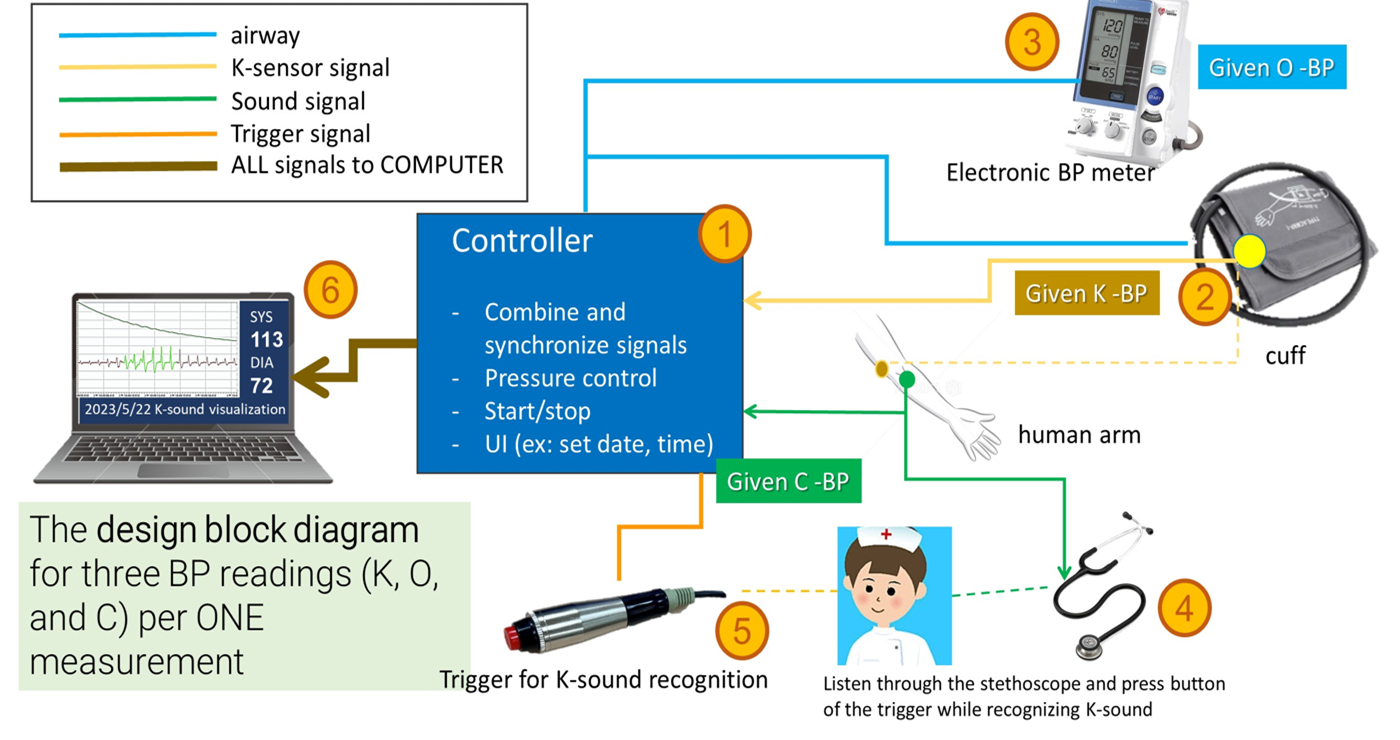
\includegraphics[keepaspectratio]{chapters/../outputs/figures/External/2-1.png}}

}

\caption[Schematic block diagram of the integrated experimental
system.]{\textbf{Schematic block diagram of the integrated experimental system.}
(1) Controller, (2) BP cuff with embedded K-Sensor, (3) oscillometric BP
device, (4) stethoscope, (5) trigger device, and (6) computer. All
signals were routed through the controller to the host computer for
real-time processing and storage, enabling simultaneous Ksens-BP,
Oscillo-BP, and Auscl-BP acquisition under identical cuff-pressure
conditions.}

\end{figure}%

\subsection{Central Controller}\label{central-controller}

A custom-designed controller based on an RL78H1D microcontroller unit
controlled cuff inflation/deflation, synchronized signal acquisition,
and supported user operations (measurement start, date/time setting, and
data review). Signals from the K-Sensor, stethoscope audio, and trigger
device were routed to the controller and forwarded to a host computer
for real-time computation, visualization, and storage.

\subsection{K-Sensor}\label{k-sensor}

The K-Sensor consisted of a semiconductor piezoresistive strain gauge
mounted on a phosphor bronze base plate (approximately 25 mm diameter x
3 mm thickness), enclosed in an aluminum frame, with a biocompatible
skin-contacting film. The sensor was embedded directly in a standard
upper-arm cuff and positioned over the brachial artery.

\begin{figure}[H]

{\centering \pandocbounded{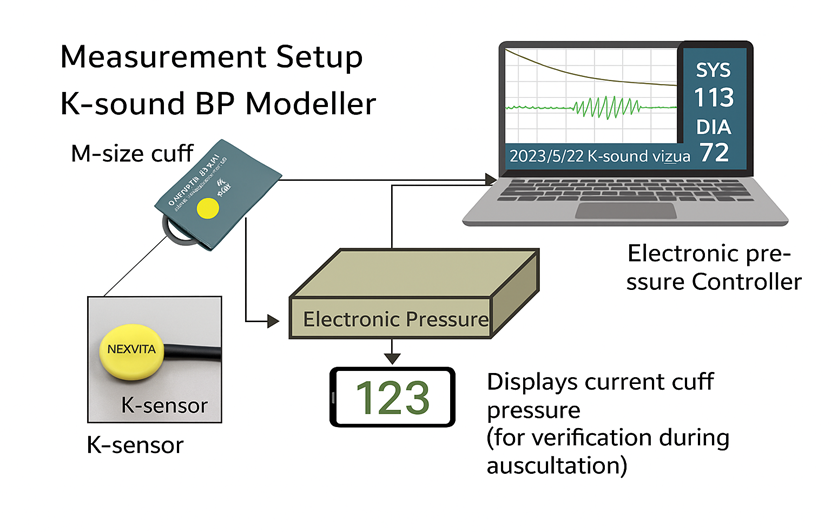
\includegraphics[keepaspectratio]{chapters/../outputs/figures/External/2-2.png}}

}

\caption[Setup of the K-Sensor BP
monitor.]{\textbf{Setup of the K-Sensor BP monitor.} During cuff
deflation, the K-Sensor continuously captures arterial wall vibrations
associated with Korotkoff sounds. The signal is transmitted to a
pretrained host-computer model to determine Ksens-BP.}

\end{figure}%

\subsection{Ksens-BP Acquisition}\label{ksens-bp-acquisition}

During each automated Ksens-BP measurement, cuff pressure and K-Sensor
vibration signals were recorded synchronously. The cuff was inflated to
a suprasystolic level and deflated in a controlled manner. A pretrained
classification model was applied to the deflation-period K-Sensor
waveform to detect Korotkoff-related segments (label 1 for Korotkoff
sound present, label 0 for absent). These labels were mapped to the
simultaneously recorded cuff-pressure trace. Ksens-SBP was defined at
the first segment labeled 1 (onset of Korotkoff sounds), and Ksens-DBP
at the last segment labeled 1 (disappearance of Korotkoff sounds). When
needed, cuff pressure at these time points was obtained by time
alignment and interpolation.

\pandocbounded{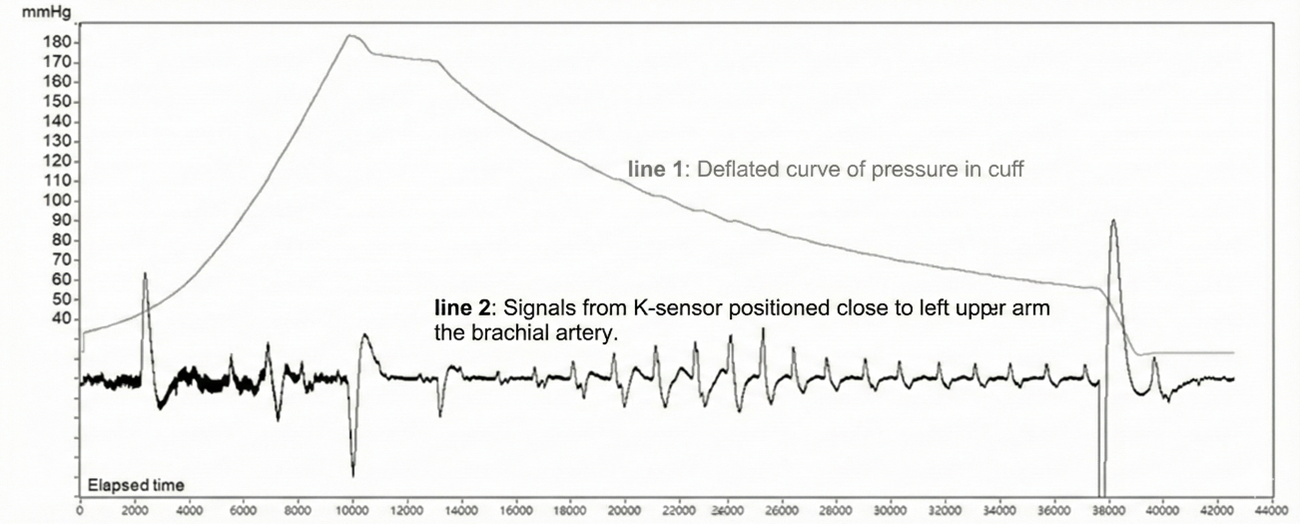
\includegraphics[keepaspectratio]{chapters/../outputs/figures/External/2-3a.png}}

\pandocbounded{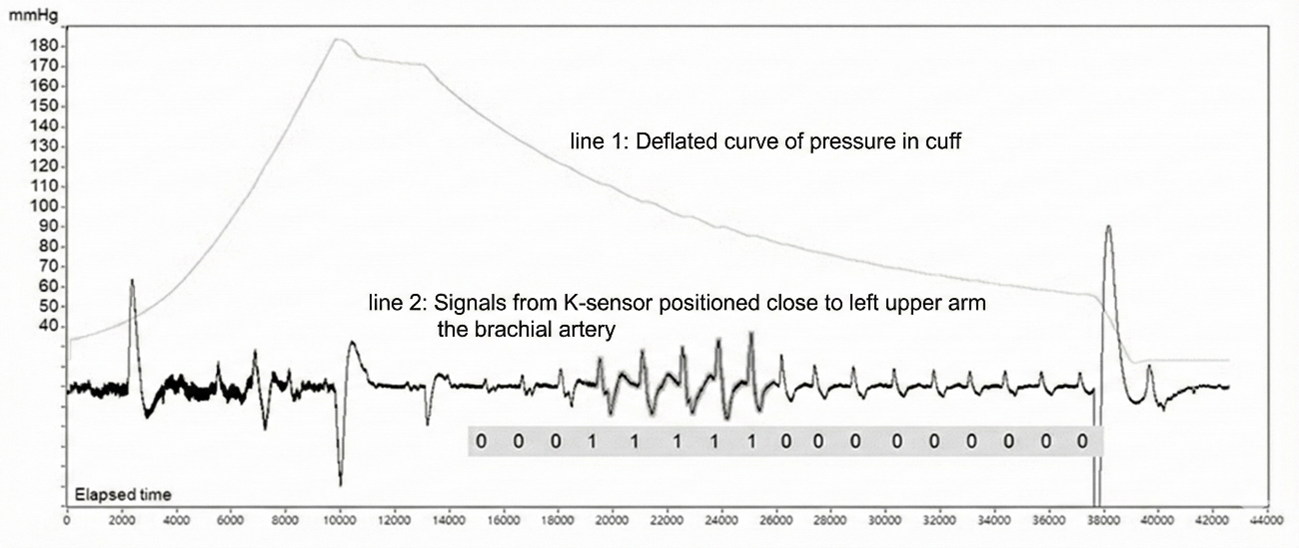
\includegraphics[keepaspectratio]{chapters/../outputs/figures/External/2-3b.png}}

\begin{figure}[H]

{\centering \pandocbounded{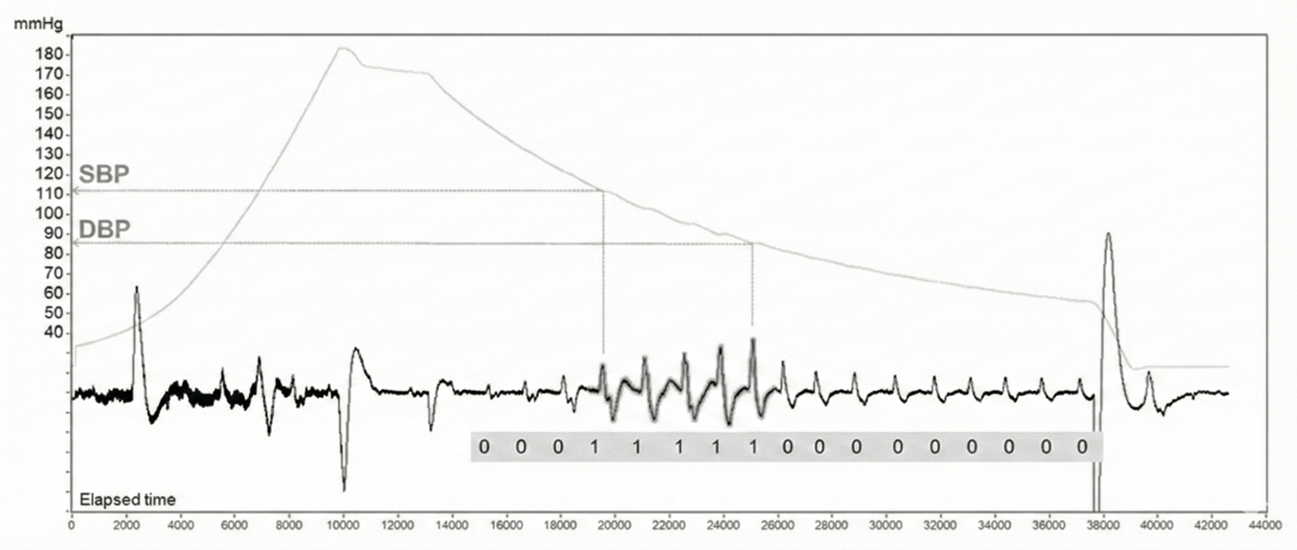
\includegraphics[keepaspectratio]{chapters/../outputs/figures/External/2-3c.png}}

}

\caption[Schematic diagram of the Ksens-BP determination
process.]{\textbf{Schematic diagram of the Ksens-BP determination
process.} Panel (a): Representative recording of cuff pressure during
inflation/deflation and the simultaneously acquired K-Sensor waveform.
Panel (b): Automated discrimination of Korotkoff-related pulses within
the K-Sensor signal during cuff deflation. Panel (c): SBP and DBP are
derived by mapping cuff pressure at the first and last detected
Korotkoff pulses, respectively.}

\end{figure}%

\subsection{Oscillometric Device
Integration}\label{oscillometric-device-integration}

An Omron HEM-907 fully automated oscillometric sphygmomanometer (Omron
Healthcare, Kyoto, Japan) was used as the oscillometric comparator. The
Omron tubing was connected to the same cuff with embedded K-Sensor to
ensure identical cuff pressure conditions. Oscillo-BP values were read
from the device after deflation and recorded by research staff.

\subsection{Auscultatory BP}\label{auscultatory-bp}

A standard medical-grade stethoscope diaphragm was positioned over the
antecubital fossa and fixed with an elastic strap. The stethoscope
acoustic signal was routed through a bifurcated circuit and converted to
an electrical signal for controller input. During each measurement,
trained healthcare personnel listened to Korotkoff sounds and pressed a
handheld trigger button for each detected Korotkoff sound, from first
sound (SBP) to last sound (DBP). The host computer automatically
recorded Auscl-BP values according to trigger timing and corresponding
cuff pressure.

To minimize bias, the auscultating healthcare professional and the
host-computer operator were separated. The auscultating professional was
blinded to real-time signals and computed BP values.

\section{Experimental Protocol}\label{experimental-protocol}

All measurements were performed in a quiet, temperature-controlled room,
with participants seated and rested for at least 5 minutes before data
collection. The sequence was:

\begin{enumerate}
\def\labelenumi{\arabic{enumi}.}
\tightlist
\item
  Cuff inflation to 180 mmHg (or higher if baseline BP exceeded this
  level).
\item
  Controlled deflation at approximately 5 mmHg/s.
\item
  During deflation, simultaneous K-Sensor signal recording and
  auscultatory trigger marking for Ksens-BP and Auscl-BP derivation.
\item
  After complete deflation, on-screen Oscillo-BP values were recorded.
\item
  Three consecutive measurements per participant with a 1-minute rest
  interval; failed measurements were repeated, allowing up to five
  attempts.
\end{enumerate}

\begin{figure}[H]

{\centering \pandocbounded{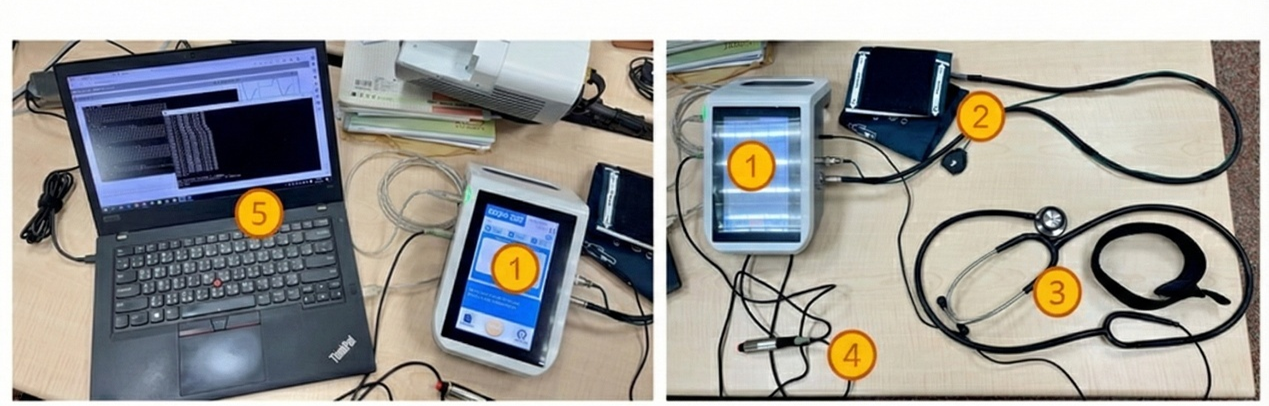
\includegraphics[keepaspectratio]{chapters/../outputs/figures/External/2-4.png}}

}

\caption[Actual equipment setup and signal acquisition
workflow.]{\textbf{Actual equipment setup and signal acquisition workflow for the automated K-sound blood pressure monitoring system.}
Left panel: integrated platform with central controller (Label 1)
streaming synchronized signals to a laptop (Label 5) for automated
K-sound detection and Ksens-BP estimation, with Auscl-BP displayed for
reference. Right panel: measurement components and controller inputs,
including cuff pressure, stethoscope audio (Label 3), K-Sensor signal
(Label 2), and operator trigger signal (Label 4).}

\end{figure}%

\section{Statistical Analysis}\label{statistical-analysis}

All analyses were performed in R (Version 4.5.2) (R Foundation for
Statistical Computing, Vienna, Austria). Continuous variables are
presented as mean +/- SD and categorical variables as n (\%).

Agreement between devices and the auscultatory reference was evaluated
using Lin's CCC with 95\% confidence intervals and Bland-Altman analysis
(mean bias and 95\% limits of agreement). Method differences were
summarized by mean difference, SD, and mean absolute difference, and
absolute errors were compared using paired Wilcoxon signed-rank tests.

Factors associated with measurement differences were assessed using
linear mixed-effects models with participant-level random intercepts.
Subgroup analyses were also performed using mixed-effects models with
estimated marginal means.

Oscillo-BP error was analyzed at attempt and patient levels using
descriptive comparisons --- including standardized mean difference (SMD)
to quantify covariate imbalance --- and logistic regression models
(mixed-effects logistic model for attempt-level data and standard
logistic model for patient-level data). Odds ratios with 95\% confidence
intervals are reported. All tests were two-sided, and p \textless{} 0.05
was considered statistically significant.

\bookmarksetup{startatroot}

\chapter{Results}\label{results}

\section{Study Population}\label{study-population-1}

\begin{figure}[H]

{\centering 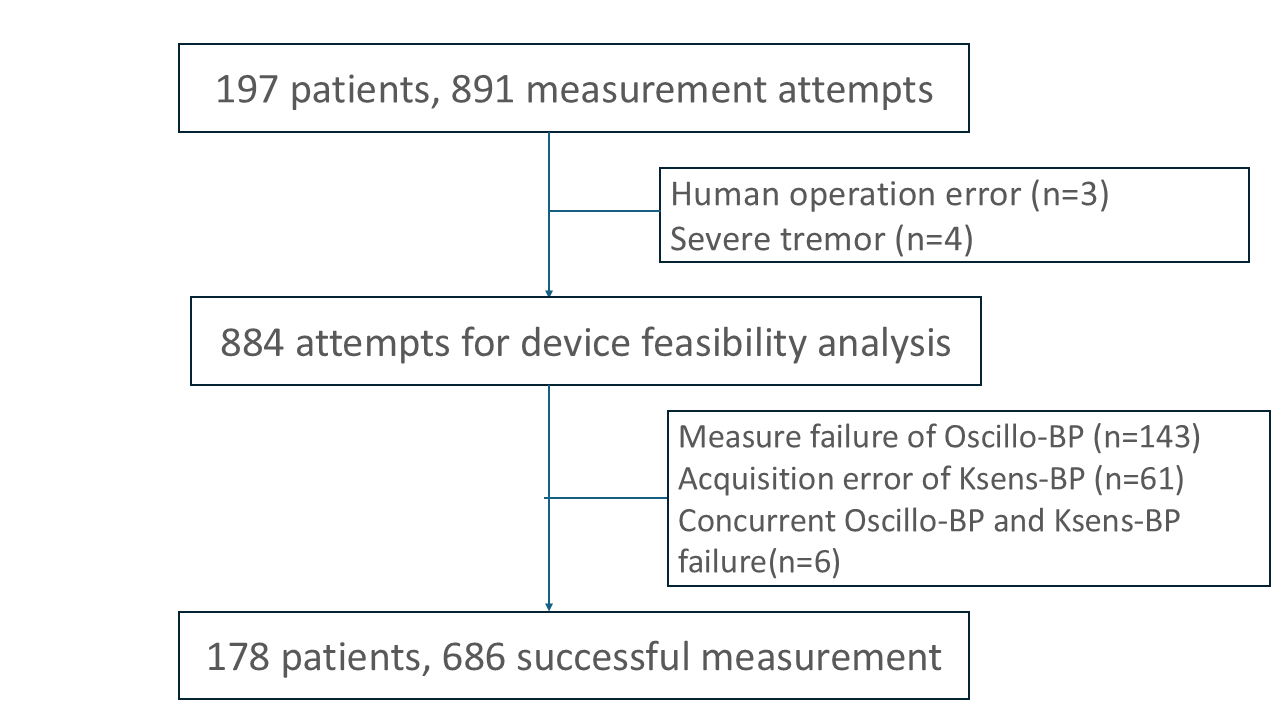
\includegraphics[width=\linewidth,height=0.85\textheight,keepaspectratio]{chapters/../outputs/figures/3-1.png}

}

\caption[Study flow from enrollment to the final paired analytic
dataset.]{\textbf{Study flow from enrollment to the final paired
analytic dataset.}}

\end{figure}%

\FloatBarrier

As shown in Figure 3.1, a total of 197 patients contributed 891 blood
pressure measurement attempts during the study period. Seven attempts
were excluded before device feasibility analysis because of human
operation error (n = 3) or severe tremor (n = 4), leaving 884 attempts
for feasibility evaluation. Among these, additional attempts were
excluded due to Oscillo-BP measurement failure (n = 143), Ksens-BP
acquisition error (n = 61), or concurrent failure of both devices (n =
6). The final analytic dataset therefore comprised 686 successful paired
measurements from 178 patients.

\FloatBarrier

\begin{table}
\caption{Baseline characteristics of the study population.}\tabularnewline

\fontsize{12.0pt}{14.0pt}\selectfont
\begin{tabular*}{\linewidth}{@{\extracolsep{\fill}}lr}
\toprule
{\bfseries Variable} & {\bfseries mean +/- SD or n(\%)} \\ 
\midrule\addlinespace[2.5pt]
{\itshape Demographics} &  \\ 
Age, years & 67.39 ± 9.61 \\ 
Sex & 142 (79.8\%) \\ 
{\itshape Anthropometrics} &  \\ 
Height, cm & 164.15 ± 8.05 \\ 
Weight, kg & 71.43 ± 13.52 \\ 
BMI, kg/m2 & 26.38 ± 3.89 \\ 
{\itshape Comorbidities} &  \\ 
HTN & 129 (72.5\%) \\ 
DM & 69 (38.8\%) \\ 
CAD & 90 (50.6\%) \\ 
AMI & 61 (34.3\%) \\ 
Stroke & 7 (3.9\%) \\ 
HF & 27 (15.2\%) \\ 
AF & 28 (15.7\%) \\ 
PAD & 6 (3.4\%) \\ 
\bottomrule
\end{tabular*}
\end{table}

Table 3.1 summarizes the baseline characteristics of the enrolled
cohort. The mean age was 67.39 +/- 9.61 years, and 142 participants
(79.8\%) were male. The mean height, body weight, and BMI were 164.15
+/- 8.05 cm, 71.43 +/- 13.52 kg, and 26.38 +/- 3.89 kg/m2, respectively.
Hypertension was the most prevalent comorbidity (129, 72.5\%), followed
by CAD (90, 50.6\%), DM (69, 38.8\%), and a history of acute MI (61,
34.3\%). HF and AF were present in 27 (15.2\%) and 28 (15.7\%)
participants, whereas stroke (7, 3.9\%) and PAD (6, 3.4\%) were less
common.

\clearpage

\section{Agreement and Systematic Differences Between
Devices}\label{agreement-and-systematic-differences-between-devices}

Table 3.2 demonstrates strong agreement between each index device and
the auscultatory reference, with consistently higher concordance for
Ksens-BP than for Oscillo-BP. For systolic blood pressure, the CCC was
0.957 (95\% CI, 0.950-0.962) for K-SYS versus C-SYS and 0.903 (95\% CI,
0.888-0.916) for O-SYS versus C-SYS. A similar pattern was observed for
diastolic blood pressure, with CCC values of 0.946 (95\% CI,
0.937-0.953) for K-DIA versus C-DIA and 0.851 (95\% CI, 0.831-0.869) for
O-DIA versus C-DIA.

\begin{table}
\caption{Agreement metrics between devices.}\tabularnewline

\fontsize{12.0pt}{14.0pt}\selectfont
\begin{tabular*}{\linewidth}{@{\extracolsep{\fill}}lr}
\toprule
{\bfseries device comparison} & {\bfseries CCC (95\% CI)} \\ 
\midrule\addlinespace[2.5pt]
{\bfseries SBP} &  \\ 
Oscillo vs. Auscl & 0.903 [0.888, 0.916] \\ 
Ksens vs. Auscl & 0.957 [0.950, 0.962] \\ 
{\bfseries DBP} &  \\ 
Oscillo vs. Auscl & 0.851 [0.831, 0.869] \\ 
Ksens vs. Auscl & 0.946 [0.937, 0.953] \\ 
\bottomrule
\end{tabular*}
\end{table}

\FloatBarrier

\begin{figure}[H]

{\centering 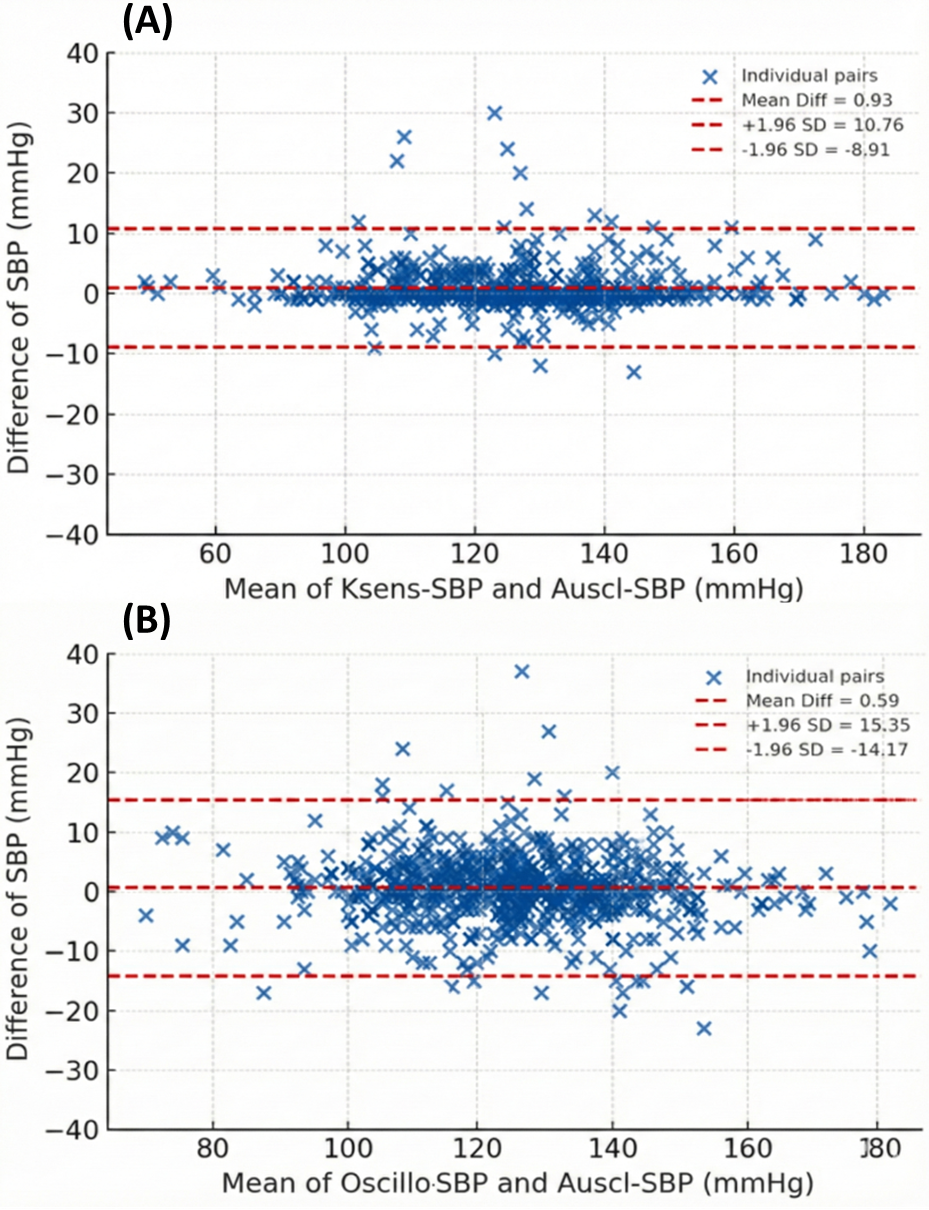
\includegraphics[width=1\linewidth,height=\textheight,keepaspectratio]{chapters/../outputs/figures/3-2.png}

}

\caption[Bland-Altman plots for systolic
BP.]{\textbf{Bland-Altman plots for systolic BP.} Panel (A): Oscillo-BP
versus auscultatory reference. Panel (B): Ksens-BP versus auscultatory
reference.}

\end{figure}%

\begin{figure}[H]

{\centering 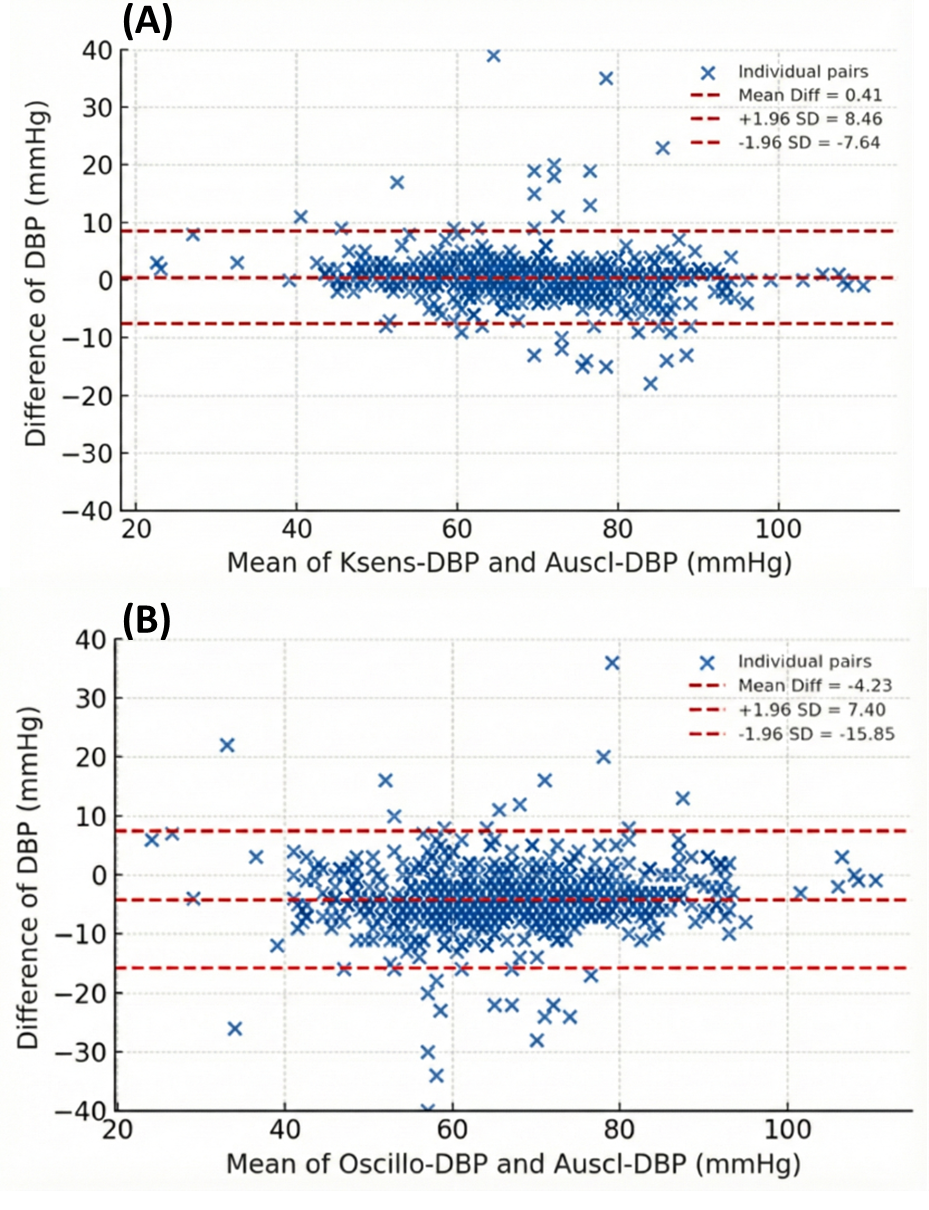
\includegraphics[width=1\linewidth,height=\textheight,keepaspectratio]{chapters/../outputs/figures/3-3.png}

}

\caption[Bland-Altman plots for diastolic
BP.]{\textbf{Bland-Altman plots for diastolic BP.} Panel (A): Oscillo-BP
versus auscultatory reference. Panel (B): Ksens-BP versus auscultatory
reference.}

\end{figure}%

\FloatBarrier

Bland-Altman plots (Figures 3.2A, 3.2B, 3.3A, and 3.3B) were concordant
with these results. For systolic pressure, Ksens-BP showed a small
positive bias with narrower limits of agreement (mean difference, 0.93
mmHg; limits of agreement, -8.91 to 10.76 mmHg) compared with Oscillo-BP
(mean difference, 0.59 mmHg; limits of agreement, -14.17 to 15.35 mmHg).
For diastolic pressure, Ksens-BP again demonstrated tighter dispersion
and minimal bias (mean difference, 0.41 mmHg; limits of agreement, -7.64
to 8.46 mmHg), whereas Oscillo-BP showed a larger negative bias and
wider limits (mean difference, -4.23 mmHg; limits of agreement, -15.85
to 7.40 mmHg), indicating systematic underestimation relative to
auscultatory measurements.

\begin{table}
\caption{Systematic differences and absolute differences.}\tabularnewline

\fontsize{10.0pt}{13.0pt}\selectfont
\begin{tabular*}{1\linewidth}{@{\extracolsep{\fill}}lrrrr}
\toprule
{\bfseries Comparison} & {\bfseries Mean of
absolute differences} & {\bfseries Mean
differences} & {\bfseries SD} & {\bfseries P value} \\ 
\midrule\addlinespace[2.5pt]
Oscillo-SYS – Auscl-SYS & 4.4 & 0.6 & 7.5 &  \\ 
Ksens-SYS – Auscl-SYS & 2.0 & 0.9 & 5.0 & < 0.001 \\ 
Oscillo-DIA – Auscl-DIA & 5.4 & -4.2 & 5.9 &  \\ 
Ksens-DIA – Auscl-DIA & 2.3 & 0.4 & 4.1 & < 0.001 \\ 
\bottomrule
\end{tabular*}
\end{table}

Consistent with the agreement analyses, Table 3.3 showed smaller
absolute differences for Ksens-BP than for Oscillo-BP in both pressure
domains. For systolic measurements, the mean absolute difference was 2.0
mmHg for Ksens-BP versus 4.4 mmHg for Oscillo-BP; for diastolic
measurements, the corresponding values were 2.3 and 5.4 mmHg. Mean
signed differences further indicated directionality of bias: Oscillo-BP
was near-neutral for systolic pressure (+0.6 mmHg) but substantially
underestimated diastolic pressure (-4.2 mmHg), whereas Ksens-BP remained
close to zero for both systolic (+0.9 mmHg) and diastolic (+0.4 mmHg)
readings. The between-device comparisons favored Ksens-BP for both
systolic and diastolic performance (both p \textless{} 0.001).

\clearpage

\section{Factors Influencing Measurement
Differences}\label{factors-influencing-measurement-differences}

\begin{table}
\caption{Mixed-effects model for systolic BP difference.}\tabularnewline

\fontsize{12.0pt}{14.0pt}\selectfont
\begin{tabular*}{\linewidth}{@{\extracolsep{\fill}}lrrrr}
\toprule
{\bfseries Variable} & {\bfseries Oscillo-SBP (95\% CI)} & {\bfseries p} & {\bfseries Ksens-SBP (95\% CI)} & {\bfseries p} \\ 
\midrule\addlinespace[2.5pt]
Age (per year) & 0.00 (-0.08, 0.09) & 0.91 & 0.03 (-0.01, 0.07) & 0.16 \\ 
Male sex & 2.92 (1.00, 4.84) & 0.00 & -0.03 (-1.03, 0.98) & 0.96 \\ 
Af & -1.72 (-3.99, 0.55) & 0.14 & -0.01 (-1.22, 1.20) & 0.99 \\ 
HR (per bpm) & -0.02 (-0.07, 0.04) & 0.57 & 0.00 (-0.03, 0.03) & 0.93 \\ 
HTN & -1.14 (-2.88, 0.60) & 0.20 & 0.42 (-0.48, 1.32) & 0.36 \\ 
DM & 0.94 (-0.59, 2.47) & 0.23 & -0.75 (-1.56, 0.06) & 0.07 \\ 
ASCVD & -0.44 (-2.03, 1.15) & 0.59 & 0.16 (-0.66, 0.99) & 0.70 \\ 
\bottomrule
\end{tabular*}
\end{table}

\begin{table}
\caption{Mixed-effects model for diastolic BP difference.}\tabularnewline

\fontsize{12.0pt}{14.0pt}\selectfont
\begin{tabular*}{\linewidth}{@{\extracolsep{\fill}}lrrrr}
\toprule
{\bfseries Variable} & {\bfseries Oscillo-DBP (95\% CI)} & {\bfseries p} & {\bfseries Ksens-DBP (95\% CI)} & {\bfseries p} \\ 
\midrule\addlinespace[2.5pt]
Age (per year) & 0.05 (-0.04, 0.14) & 0.27 & 0.00 (-0.04, 0.05) & 0.87 \\ 
Male sex & -0.77 (-2.88, 1.35) & 0.48 & -0.55 (-1.66, 0.57) & 0.34 \\ 
Af & 2.26 (-0.17, 4.69) & 0.07 & 0.02 (-1.30, 1.33) & 0.98 \\ 
HR (per bpm) & 0.04 (-0.01, 0.09) & 0.13 & -0.03 (-0.06, 0.00) & 0.05 \\ 
HTN & -0.36 (-2.28, 1.56) & 0.71 & 0.65 (-0.35, 1.66) & 0.21 \\ 
DM & 0.98 (-0.58, 2.54) & 0.22 & 0.25 (-0.64, 1.13) & 0.58 \\ 
ASCVD & -1.34 (-3.08, 0.41) & 0.13 & 0.25 (-0.67, 1.17) & 0.59 \\ 
\bottomrule
\end{tabular*}
\end{table}

Tables 3.4 and 3.5 summarize mixed-effects models evaluating clinical
factors associated with measurement differences versus the auscultatory
reference. For systolic differences (Table 3.4), male sex was
independently associated with larger Oscillo-SBP differences (beta =
2.92 mmHg, 95\% CI 1.00 to 4.84; p = 0.003), whereas no corresponding
association was observed for Ksens-SBP (beta = -0.03 mmHg, 95\% CI -1.03
to 0.98; p = 0.959). No other covariates reached statistical
significance for systolic differences in either device model, although
DM showed a borderline inverse association in the Ksens-SBP model (beta
= -0.75 mmHg, 95\% CI -1.56 to 0.06; p = 0.070).

For diastolic differences (Table 3.5), none of the prespecified
covariates were statistically significant at the 0.05 level in either
device model. In the Ksens-DBP model, higher heart rate (HR) showed a
borderline negative association with measurement differences (beta =
-0.03 mmHg per bpm, 95\% CI -0.06 to 0.00; p = 0.052). In the
Oscillo-DBP model, AF tended to be associated with larger positive
differences (beta = 2.26 mmHg, 95\% CI -0.17 to 4.69; p = 0.069), but
this did not reach conventional significance. Overall, these findings
suggest limited and outcome-specific covariate effects, with the most
robust signal observed for sex-related variation in Oscillo-based
systolic measurements.

\clearpage

\section{Subgroup Analyses}\label{subgroup-analyses}

\begin{figure}[H]

\centering{


\includegraphics[width=1\linewidth,height=\textheight,keepaspectratio]{chapters/../outputs/figures/3-4forest_SYS_absdiff_subgroups.png}

}

\caption[Forest plot of subgroup analyses for systolic absolute
differences.]{\label{fig-forest-sbp}\textbf{Forest plot of subgroup
analyses for systolic absolute differences.} Subgroup-specific estimates
of mean absolute systolic BP differences between Ksens-BP and Oscillo-BP
versus the auscultatory reference.}

\end{figure}%

\begin{figure}[H]

\centering{


\includegraphics[width=1\linewidth,height=\textheight,keepaspectratio]{chapters/../outputs/figures/3-5forest_DIA_absdiff_subgroups.png}

}

\caption[Forest plot of subgroup analyses for diastolic absolute
differences.]{\label{fig-forest-dbp}\textbf{Forest plot of subgroup
analyses for diastolic absolute differences.} Subgroup-specific
estimates of mean absolute diastolic BP differences between Ksens-BP and
Oscillo-BP versus the auscultatory reference.}

\end{figure}%

Figures 3.4 and 3.5 summarize subgroup analyses of comparative device
performance across hypertension, DM, other ASCVD, PAD, AF, and HR
strata. For systolic absolute error (Figure 3.4), the subgroup-specific
estimates were consistently below zero, indicating that Ksens-BP
maintained smaller absolute systolic deviation from the auscultatory
reference than Oscillo-BP across all prespecified subgroups. No
significant between-level contrasts were observed for systolic outcomes
(all p \textgreater{} 0.05), suggesting no strong effect modification.

For diastolic absolute error (Figure 3.5), the overall pattern also
favored Ksens-BP, but heterogeneity was evident in selected subgroups.
Significant subgroup differences were observed for DM (Yes vs No: beta =
-1.52 mmHg, 95\% CI -2.76 to -0.28; p = 0.016) and PAD (Yes vs No: beta
= 5.07 mmHg, 95\% CI 1.59 to 8.55; p = 0.005), whereas contrasts by
hypertension, other ASCVD, and AF were not significant. Although the
formal HR tertile analysis did not reach statistical significance, a
directional trend toward larger diastolic differences at higher HR was
visually apparent in the forest plot. A post-hoc binary analysis using a
clinically relevant threshold (HR \textless{} 100 vs ≥ 100 bpm)
confirmed a significant interaction (mean difference 5.48 {[}95\% CI,
3.59--7.37{]} vs 8.43 {[}95\% CI, 5.36--11.50{]} mmHg; p for interaction
= 0.022), suggesting that the diastolic accuracy advantage of Ksens-BP
over Oscillo-BP was amplified in patients with elevated HR. These
findings indicate that the comparative diastolic advantage of Ksens-BP
was generally robust but varied in magnitude according to specific
comorbidity and hemodynamic profiles.

\clearpage

\section{Omron Error Analysis}\label{omron-error-analysis}

\begin{table}
\caption{Omron error descriptive summary (attempt-level).}\tabularnewline

\fontsize{10.0pt}{13.0pt}\selectfont
\begin{tabular*}{1\linewidth}{@{\extracolsep{\fill}}lllrr}
\toprule
{\bfseries Variable} & {\bfseries Error} & {\bfseries No error} & {\bfseries Difference
[95\% CI]} & {\bfseries SMD} \\ 
\midrule\addlinespace[2.5pt]
Age (years) & 69.18 ± 9.45 & 67.05 ± 9.51 & 2.13 (0.43, 3.83) & 0.22 \\ 
Arm circumference (cm) & 25.93 ± 3.16 & 27.07 ± 3.18 & -1.14 (-1.71, -0.57) & -0.36 \\ 
BMI (kg/m\textasciicircum{}2) & 25.15 ± 4.11 & 26.47 ± 3.96 & -1.31 (-2.05, -0.58) & -0.33 \\ 
Heart rate (bpm) & 78.01 ± 18.05 & 72.49 ± 14.13 & 5.52 (2.37, 8.67) & 0.37 \\ 
Male sex & 104 (72.73\%) & 589 (79.49\%) & -0.07 (-0.15, 0.01) & -0.16 \\ 
Hypertension & 101 (70.63\%) & 532 (71.79\%) & -0.01 (-0.09, 0.07) & -0.03 \\ 
Diabetes mellitus & 43 (30.07\%) & 299 (40.35\%) & -0.10 (-0.19, -0.02) & -0.22 \\ 
Atrial fibrillation & 57 (39.86\%) & 95 (12.82\%) & 0.27 (0.19, 0.35) & 0.65 \\ 
Heart failure & 31 (21.68\%) & 106 (14.30\%) & 0.07 (0.00, 0.15) & 0.19 \\ 
Peripheral artery disease & 15 (10.49\%) & 21 (2.83\%) & 0.08 (0.02, 0.13) & 0.31 \\ 
ASCVD (any) & 67 (46.85\%) & 431 (58.16\%) & -0.11 (-0.20, -0.02) & -0.23 \\ 
\bottomrule
\end{tabular*}
\begin{minipage}{\linewidth}
\vspace{.05em}
SMD, standardized mean difference.\\
\end{minipage}
\end{table}

\begin{table}
\caption{Omron error descriptive summary (patient-level).}\tabularnewline

\fontsize{10.0pt}{13.0pt}\selectfont
\begin{tabular*}{1\linewidth}{@{\extracolsep{\fill}}lllrr}
\toprule
{\bfseries Variable} & {\bfseries Error} & {\bfseries No error} & {\bfseries Difference
[95\% CI]} & {\bfseries SMD} \\ 
\midrule\addlinespace[2.5pt]
Age (years) & 70.72 ± 8.92 & 65.67 ± 9.68 & 5.06 (2.31, 7.81) & 0.54 \\ 
Arm circumference (cm) & 25.90 ± 3.24 & 27.50 ± 3.06 & -1.60 (-2.55, -0.64) & -0.51 \\ 
BMI (kg/m\textasciicircum{}2) & 25.08 ± 3.93 & 27.05 ± 3.86 & -1.96 (-3.13, -0.79) & -0.51 \\ 
Heart rate (bpm) & 76.02 ± 17.11 & 72.15 ± 12.92 & 3.86 (-0.90, 8.63) & 0.27 \\ 
Male sex & 48 (73.85\%) & 108 (81.82\%) & -0.08 (-0.21, 0.05) & -0.19 \\ 
Hypertension & 44 (67.69\%) & 98 (74.24\%) & -0.07 (-0.20, 0.07) & -0.14 \\ 
Diabetes mellitus & 21 (32.31\%) & 56 (42.42\%) & -0.10 (-0.24, 0.04) & -0.21 \\ 
Atrial fibrillation & 22 (33.85\%) & 10 (7.58\%) & 0.26 (0.14, 0.39) & 0.69 \\ 
Heart failure & 14 (21.54\%) & 17 (12.88\%) & 0.09 (-0.03, 0.20) & 0.23 \\ 
Peripheral artery disease & 5 (7.69\%) & 3 (2.27\%) & 0.05 (-0.02, 0.12) & 0.25 \\ 
ASCVD (any) & 35 (53.85\%) & 75 (56.82\%) & -0.03 (-0.18, 0.12) & -0.06 \\ 
\bottomrule
\end{tabular*}
\begin{minipage}{\linewidth}
\vspace{.05em}
SMD, standardized mean difference.\\
\end{minipage}
\end{table}

Tables 3.6 and 3.7 show a consistent risk profile for Omron measurement
error at both the attempt and patient levels. Compared with non-error
observations, error events were associated with older age, smaller arm
circumference, lower BMI, and higher HR, with the largest standardized
imbalance observed for AF. At the attempt level, AF was substantially
more frequent in error attempts (39.9\% vs 12.8\%; SMD = 0.65), and
similar enrichment was observed at the patient level (33.9\% vs 7.6\%;
SMD = 0.69). PAD was also more prevalent among error attempts, whereas
DM and composite ASCVD were less frequent in the error group.

\begin{table}
\caption{Mixed-effects logistic regression for Omron error (attempt-level).}\tabularnewline

\fontsize{12.0pt}{14.0pt}\selectfont
\begin{tabular*}{\linewidth}{@{\extracolsep{\fill}}lrl}
\toprule
{\bfseries Predictor} & {\bfseries OR (95\% CI)} & {\bfseries p} \\ 
\midrule\addlinespace[2.5pt]
Atrial fibrillation (Yes vs No) & 13.35 (3.00-59.45) & <0.001 \\ 
Age (per 1 SD) & 1.31 (0.73-2.36) & 0.366 \\ 
Heart rate (per 1 SD) & 1.58 (0.97-2.55) & 0.064 \\ 
Arm circumference (per 1 SD) & 0.64 (0.36-1.14) & 0.132 \\ 
Male (ref: Female) & 0.57 (0.16-2.08) & 0.397 \\ 
Peripheral artery disease (Yes vs No) & 6.37 (0.46-87.34) & 0.166 \\ 
\bottomrule
\end{tabular*}
\end{table}

\begin{table}
\caption{Logistic regression for Omron error (patient-level).}\tabularnewline

\fontsize{12.0pt}{14.0pt}\selectfont
\begin{tabular*}{\linewidth}{@{\extracolsep{\fill}}lrl}
\toprule
{\bfseries Predictor} & {\bfseries OR (95\% CI)} & {\bfseries p} \\ 
\midrule\addlinespace[2.5pt]
Atrial fibrillation (Yes vs No) & 4.63 (1.91-11.24) & <0.001 \\ 
Age (per 1 SD) & 1.52 (1.04-2.22) & 0.029 \\ 
Heart rate (per 1 SD) & 1.33 (0.94-1.88) & 0.108 \\ 
Arm circumference (per 1 SD) & 0.72 (0.50-1.02) & 0.064 \\ 
Male (ref: Female) & 0.62 (0.28-1.35) & 0.228 \\ 
\bottomrule
\end{tabular*}
\end{table}

Multivariable regression analyses (Tables 3.8 and 3.9) identified AF as
the most robust independent correlate of Omron error. In the
mixed-effects attempt-level model, AF was associated with markedly
increased odds of error (odds ratio {[}OR{]}, 13.35; 95\% CI,
3.00-59.45; p \textless{} 0.001), while age, HR, arm circumference, sex,
and PAD were not statistically significant after adjustment. In the
patient-level logistic model, AF remained strongly associated with error
(OR, 4.63; 95\% CI, 1.91-11.24; p \textless{} 0.001), and older age also
emerged as an independent predictor (OR per 1 SD, 1.52; 95\% CI,
1.04-2.22; p = 0.029). Smaller arm circumference showed a borderline
inverse association (OR per 1 SD, 0.72; 95\% CI, 0.50-1.02; p = 0.064),
and HR remained directionally positive but non-significant.

\bookmarksetup{startatroot}

\chapter{Discussion}\label{discussion}

\section{Principal Findings}\label{principal-findings}

In this cardiovascular outpatient cohort, Ksens-BP demonstrated higher
concordance with the auscultatory reference than Oscillo-BP across both
pressure domains, with roughly half the absolute error and substantially
narrower limits of agreement. Oscillo-BP additionally showed a
systematic 4.2 mmHg diastolic underestimation that was absent in
Ksens-BP. Mixed-effects models identified male sex as an independent
predictor of larger Oscillo-SBP discrepancy, with no corresponding
effect on Ksens-SBP --- a dissociation that persisted after adjustment
for other covariates. Subgroup analyses showed that the systolic
agreement advantage of Ksens-BP was consistent across all prespecified
clinical subgroups. For diastolic performance, the pattern was generally
maintained but varied by comorbidity: the Ksens advantage was augmented
in PAD patients and attenuated in those with DM, the two subgroups with
the most significant interaction terms.

A separate line of analysis addressed oscillometric device failure
rather than agreement. AF was the dominant independent predictor of
Omron measurement failure, with an adjusted odds ratio exceeding 13 at
the attempt level and approximately 5 at the patient level; older age
was an additional predictor in the patient-level model. These failure
rates were not captured in the agreement analysis and represent a
clinically distinct dimension of device performance.

\section{Mechanistic Basis of Ksens-BP
Superiority}\label{mechanistic-basis-of-ksens-bp-superiority}

The consistent agreement advantage of Ksens-BP across both pressure
domains and subgroups likely reflects a fundamental difference in signal
origin. Oscillometric devices derive SBP and DBP algorithmically from
cuff-transmitted pressure oscillations: MAP is identified at the peak of
the oscillometric waveform envelope, and SBP and DBP are subsequently
back-calculated using device-specific, unpublished amplitude
ratios\textsuperscript{4}. This two-step inference introduces a
structural source of error: once the OMWE peak is determined, any
deviation in the assumed ratio propagates directly into the SBP and DBP
estimates. In contrast, Ksens-BP directly identifies the cuff pressure
at the first and last detectable Korotkoff-related event, with no
algorithmic interpolation between MAP and the pressure endpoints of
interest.

The sensor mechanism is also distinct. Baranger et al.~demonstrated
using synchronized ultrafast ultrasound and stethoscope recordings that
clinically recorded K-sounds are more consistent with tissue-borne shear
vibrations transmitted through the arterial wall and surrounding soft
tissue than with compressional airborne waves radiating outward from the
brachial artery\textsuperscript{39}. The semiconductor piezoresistive
strain gauge in the K-Sensor transduces these tissue-borne
microvibrations directly, rather than detecting airborne acoustic
pressure. Semiconductor strain gauges achieve gauge factors of 100--200,
nearly two orders of magnitude greater than the 2--5 typical of
conventional metal-foil gauges\textsuperscript{40}, enabling detection
of submicron-scale arterial wall displacements that fall below the
resolution threshold of metal-based MEMS piezoresistive sensors designed
for heart sound and pulse detection\textsuperscript{41}. This
transduction principle also differs fundamentally from piezoelectric
approaches: PVDF film--based sensors have demonstrated automated K-sound
detection with high correlation to auscultatory BP\textsuperscript{27},
and wearable piezoelectret patches can record K-sounds without a
stethoscope\textsuperscript{29}, yet both piezoelectric sensor types
generate charge proportional to strain rate rather than strain itself,
inherently filtering out low-frequency waveform components and remaining
susceptible to ambient acoustic contamination\textsuperscript{42}. By
contrast, the piezoresistive element provides direct
strain-to-resistance conversion in the low-frequency, small-displacement
regime characteristic of K-sound--related arterial vibrations,
conferring enhanced coupling to the pulsatile arterial wall motion that
constitutes the clinically relevant signal while attenuating
environmental noise. The narrow limits of agreement observed in this
study (−8.91 to +10.76 mmHg systolic; −7.64 to +8.46 mmHg diastolic) are
consistent with a device whose measurement endpoints map directly onto
the physiological events that define auscultatory SBP and DBP.

\section{Systematic Diastolic Underestimation by
Oscillometry}\label{systematic-diastolic-underestimation-by-oscillometry}

The −4.23 mmHg mean diastolic bias of Oscillo-BP warrants specific
attention because it is a unidirectional, systematic offset rather than
random noise --- a pattern consistent with a structural limitation of
the fixed-ratio oscillometric algorithm in populations with elevated
arterial stiffness.

All mainstream oscillometric devices estimate DBP by applying a fixed
amplitude ratio to the OMWE peak: diastolic pressure is assigned at the
cuff pressure corresponding to a predetermined fraction of the peak
oscillation amplitude during the descending limb of deflation.
Chandrasekhar et al.~demonstrated mathematically that this fixed-ratio
approach is inherently sensitive to arterial compliance: the optimal
ratios shift substantially (by 0.5--0.6) across individuals as
compliance and pulse pressure vary, and because BP error is amplified by
a factor exceeding 40 relative to the ratio error, even modest
compliance-related deviation in the assumed ratio produces clinically
meaningful DBP inaccuracy\textsuperscript{43}. Liang et al.~confirmed
this in a computational model of brachial arterial stiffening: as
arterial stiffness increases, the descending limb of the OMWE flattens,
causing the fixed-ratio algorithm to assign diastolic pressure at a cuff
pressure point earlier and lower than the true auscultatory
endpoint\textsuperscript{7}. Raamat et al.~similarly showed via
simulation that oscillometric DBP errors are systematically directional
and stiffness-dependent\textsuperscript{14}.

This mechanistic prediction is borne out clinically. Landgraf et al., in
a cardiovascular outpatient sample, reported oscillometric DBP
underestimation relative to auscultation\textsuperscript{8}. Nedel et
al.'s meta-analysis of oscillometric versus invasive MAP in critically
ill patients --- a population with high vascular disease burden ---
found limits of agreement spanning −14.6 to +40.3 mmHg, indicating that
even when mean bias appears acceptable, individual-level diastolic
agreement is substantially degraded in high-acuity
populations\textsuperscript{9}. The present cohort, enriched with CAD
(50.6\%), DM (38.8\%), and hypertensive end-organ disease, represents
precisely the patient segment in which compliance-driven DBP ratio error
is expected to be largest.

Ksens-BP's near-zero diastolic bias (+0.41 mmHg) follows directly from
its measurement principle: DBP is read at the last detectable K-sound
event, a physiological endpoint that is independent of waveform
amplitude ratios and therefore unaffected by compliance-related
distortion of the OMWE shape.

\section{Sex-Related Variation in Oscillometric Systolic
Error}\label{sex-related-variation-in-oscillometric-systolic-error}

Male sex was independently associated with larger Oscillo-SBP
measurement differences (β = +2.92 mmHg, p = 0.003), with no
corresponding effect on Ksens-SBP (β = −0.03, p = 0.959). This pattern
is consistent with prior reports: Kim et al.~found male sex to be an
independent predictor of oscillometric--auscultatory SBP discrepancy (β
= +2.00, p \textless{} 0.0001) in the Korea National Health and
Nutrition Examination Survey\textsuperscript{44,45}, and Bhatt et
al.~demonstrated that an oscillometric device overestimated mean BP in
men and underestimated it in women even after comprehensive
multivariable adjustment\textsuperscript{46}. In the Invasive Blood
Pressure Consortium, Abbaoui et al.~quantified the total sex effect on
cuff-versus-invasive SBP discrepancy at 6.1 mmHg (95\% CI, 3.8--8.4),
with 55\% mediated by height; a residual direct effect of 2.7 mmHg
persisted after height adjustment, indicating that stature accounts for
most but not all of the difference\textsuperscript{47}.

The mechanistic basis is multifactorial. Height-related differences in
pulse wave reflection timing alter peripheral SBP amplification in a
sex-dependent manner\textsuperscript{47,48}, while age-related arterial
stiffness progression --- which is more advanced in men at this age ---
modifies the oscillometric waveform envelope in ways that deviate from
OMWE algorithm assumptions\textsuperscript{10}. Additionally, men more
frequently require large or extra-large cuffs; Ishigami et al.~showed
that cuff size mismatch alone introduces SBP errors up to +19.5 mmHg,
representing a further sex-linked error pathway\textsuperscript{49}.
That Bhatt et al.'s sex effect survived adjustment for all measurable
covariates suggests these pathways act in aggregate rather than in
isolation\textsuperscript{46}.

The Ksens result is decoupled from all of these mechanisms: K-sound
detection is anchored to arterial wall motion events rather than
oscillometric waveform morphology, and is therefore insensitive to
sex-related differences in vascular mechanics and arm anthropometry. In
older male patients --- the prototype patient at this outpatient clinic
--- oscillometric SBP readings carry an additional systematic upward
bias that a K-sound--based system avoids.

\section{Performance of Automated K-Sound
Devices}\label{performance-of-automated-k-sound-devices}

Among validated automated K-sound monitors, the agreement profile of
Ksens-BP is most directly comparable to two AAMI/ESH/ISO-validated
devices from the same technology lineage. The InBody BPBIO480KV,
validated in a general outpatient population (mean age 57.3 years),
yielded mean SBP and DBP biases of 0.3 ± 5.5 and 0.6 ± 4.7 mmHg against
simultaneous mercury auscultation\textsuperscript{20}; the KOROT V2
Doctor in a comparable general cohort (mean age 56.4 years) produced
−1.3 ± 6.0 and 1.5 ± 5.0 mmHg\textsuperscript{26}. The corresponding
figures for Ksens-BP in the present study --- SBP +0.93 mmHg and DBP
+0.41 mmHg, with SDs of approximately 5.0 and 4.1 mmHg inferred from
Bland--Altman limits of agreement --- are numerically within this range,
with near-zero mean bias and measurement dispersion below 5 mmHg in each
pressure domain.

The Hanvon FY730 and KSY8600 reported considerably narrower dispersions.
The FY730 (mean age 59.6 years) produced biases of −0.37 ± 2.25 and
−0.17 ± 2.02 mmHg\textsuperscript{36}, and the KSY8600 (mean age 51.3
years) achieved −0.4 ± 2.09 and −0.3 ± 1.86 mmHg\textsuperscript{37} ---
SDs approximately 2.5-fold lower than those seen in the InBody, KOROT,
and present study results. This apparent precision advantage most
plausibly reflects participant characteristics rather than sensor
superiority. Both Hanvon studies enrolled younger adults without
arrhythmia, recruited specifically to satisfy ISO arm circumference and
BP distribution criteria in low-risk settings. Younger, physiologically
homogeneous participants exhibit lower intra-individual BP variability
and produce more consistent K-sound signals --- both of which reduce
observed measurement SD independently of device performance. Whether
either Hanvon device maintains this precision in older or clinically
complex populations remains untested.

The critical distinction between the present study and all four
comparators is the enrolled population. ISO 81060-2 validation studies
are designed to enrol participants meeting prescribed distributions of
age, sex, arm circumference, and resting BP in a general adult sample
--- a strategy that minimises physiological heterogeneity and optimises
measurement reproducibility. The present cohort was not assembled for
validation purposes but represents real-world cardiovascular outpatient
practice: mean age 67.4 years, with CAD in 50.6\%, DM in 38.8\%, and AF
in 15.7\%. All four comparator studies excluded arrhythmia; none
enrolled a population with this comorbidity profile. That Ksens-BP
achieves SDs in the 4--5 mmHg range in this setting --- consistent with
InBody and KOROT results in healthier general populations --- indicates
that the agreement with auscultation established in standardised
validation environments extends to the clinically demanding populations
in which the device is most needed.

\section{Atrial Fibrillation as the Primary Driver of Oscillometric
Failure}\label{atrial-fibrillation-as-the-primary-driver-of-oscillometric-failure}

AF was strongly associated with oscillo-BP measurement failure. Although
AF accounted for only 15.7\% of the enrolled cohort, it contributed to
39.9\% of failed measurement attempts, corresponding to an adjusted
attempt-level OR of 13.35 (95\% CI, 3.00--59.45). At the patient level,
AF remained the strongest independent predictor of device failure (OR,
4.63; 95\% CI, 1.91--11.24), with older age emerging as a secondary
independent factor.

In contrast to our failure-rate findings, most prior studies have
primarily assessed agreement in measurements that yield an output, with
limited attention to measurement failure (no-reading) rates. In our
review of the available validation and comparative studies, we did not
identify reports that clearly quantify oscillometric measurement failure
rates in AF. This evidentiary gap is clinically relevant because
standard validation protocol typically prespecify a minimum number of
successful paired measurements; as a result, attempts that fail to
produce an output are either excluded by design or remain unreported. As
a result, statements that oscillometric devices show ``acceptable
accuracy'' in AF may overlook an important real-world limitation, that a
meaningful subset of AF measurements may terminate without any usable BP
value.

Mechanism for the elevated failure rate in AF relates to how
oscillometric algorithms derive pressure estimates from cuff
oscillations across the deflation sweep. Oscillometric algorithms
reconstruct the OMWE by fitting a smooth monotonic envelope through
beat-by-beat cuff oscillation amplitudes over a pressure range spanning
the entire deflation sweep. In sinus rhythm, each cardiac cycle at a
given cuff pressure produces an oscillation of broadly predictable
amplitude relative to adjacent cycles, enabling reliable curve fitting
and MAP identification. In AF, the irregular RR interval produces
beat-to-beat variation in diastolic filling time and consequently in
stroke volume --- superimposing a second source of amplitude modulation
on the pressure-dependent signal that the algorithm is designed to
detect\textsuperscript{17,18}. The resulting envelope is non-monotonic
and locally irregular, preventing the algorithm from identifying a
reliable peak and therefore precluding MAP estimation entirely.
K-sound--based detection circumvents this by classifying each cuff
deflation segment independently for arterial wall vibration events; SBP
and DBP are determined from the first and last labeled events, requiring
no assumptions about inter-beat amplitude regularity.

\section{Subgroup Variation in Diastolic
Agreement}\label{subgroup-variation-in-diastolic-agreement}

The diastolic agreement advantage of Ksens-BP over Oscillo-BP was
maintained across all prespecified subgroups, consistent with the
device-level difference in measurement principle described above. Among
prespecified subgroups, two interactions reached statistical
significance; an exploratory post-hoc stratification by HR identified a
third.

In PAD patients, the Ksens diastolic advantage was augmented by
approximately 5 mmHg relative to non-PAD patients (p = 0.005). This is
mechanistically coherent: PAD is characterised by medial arterial
calcification and severely reduced wall compressibility, which distorts
the OMWE by truncating oscillation amplitude and flattening the
descending limb of the envelope --- amplifying the compliance-driven DBP
ratio error that applies to all stiff vessels\textsuperscript{7,43}.
Herráiz-Adillo et al.~demonstrated directly that calcified arteries
cause oscillometric measurement failure at a substantially elevated rate
in PAD patients, and that the error pattern is directional rather than
random\textsuperscript{50}. Massmann et al.~similarly documented
degraded oscillometric performance in symptomatic PAD with significant
atherosclerosis burden\textsuperscript{13}. In contrast, K-sound
generation depends on turbulent flow at the moment of arterial
reopening, a hydraulic event that persists even in calcified, poorly
compliant vessels; K-sound--based DBP detection is therefore
structurally less sensitive to the compliance reduction that underlies
oscillometric failure in this population. The PAD subsample in the
present study was small (n = 6), so the magnitude of the interaction
carries substantial uncertainty and requires confirmation in a dedicated
PAD cohort.

In patients with DM, the Ksens advantage was modestly attenuated (p =
0.016), though the absolute difference between groups was small. Diffuse
microvascular and autonomic changes in DM may alter both K-sound
amplitude and OMWE morphology in ways that partially offset the usual
oscillometric disadvantage; the mechanism of this interaction is not
well established and warrants further investigation.

An exploratory post-hoc stratification by HR was performed after a
visual signal was observed in the tertile forest plot despite a
non-significant interaction. The Ksens diastolic advantage was augmented
at HR ≥ 100 bpm relative to HR \textless{} 100 bpm (p for interaction =
0.022). Mechanistically, higher HR shortens the diastolic interval
between beats, reducing the number of oscillations available for OMWE
fitting and distorting the descending limb from which DBP is
estimated\textsuperscript{43}. K-sound--based detection is not affected,
as DBP is anchored to the last detected arterial vibration event
regardless of inter-beat interval. This finding should be interpreted
with caution given that the HR ≥ 100 bpm subgroup comprised only 24
attempts.

\section{Limitations}\label{limitations}

Several limitations of this study should be acknowledged. First, the
study was conducted at a single center, and the cohort was predominantly
male (80\%), which may limit the generalizability of our findings to a
broader and more diverse population. In addition, pregnant women and
pediatric patients were not included, further restricting the
applicability of the results across different demographic groups.
Second, while manual auscultation is the accepted non-invasive gold
standard, it is subject to inherent limitations such as inter-observer
variability and auditory perception thresholds. Although we employed an
integrated trigger system to standardize the capture of Auscl-BP and
minimize operation errors, this method is not as definitive as invasive
intra-arterial pressure measurement, which remains the ultimate
reference. Third, while the K-Sensor system demonstrated strong overall
performance, the exclusion of 61 measurements due to system-related
errors highlights the need for continued refinement of both the hardware
and AI algorithm to enhance reliability and reduce the likelihood of
measurement failures in clinical practice. Finally, arterial stiffness
indices (e.g., pulse wave velocity or augmentation index) were not
measured, preventing a quantitative analysis of the relationship between
arterial compliance and measurement error within the study cohort.

\bookmarksetup{startatroot}

\chapter{Conclusion}\label{conclusion}

In this cardiovascular outpatient cohort characterized by a high
prevalence of atherosclerotic comorbidities, the semiconductor
piezoresistive K-Sensor system achieved substantially better agreement
with auscultatory blood pressure than a validated oscillometric device
across both systolic and diastolic pressure domains, with particular
advantage in diastolic agreement and sex-independent measurement
consistency. Oscillometric blood pressure showed a systematic diastolic
underestimation consistent with the known sensitivity of fixed-ratio
algorithms to arterial stiffness --- a bias absent in the K-Sensor
system, which derives its pressure endpoints directly from detected
K-sound events rather than from waveform envelope interpolation. For
patients with AF --- a population in whom accurate blood pressure
control is clinically imperative --- oscillometric measurement failure
rates were prohibitively high under real-world conditions, whereas
K-sound--based detection remained viable as an endpoint detection
strategy insensitive to cardiac rhythm irregularity. These findings
position the K-Sensor approach as a technically and clinically distinct
alternative to oscillometry for patient populations in whom the
oscillometric measurement model is structurally compromised, including
those with AF and advanced atherosclerosis.

\bookmarksetup{startatroot}

\chapter{Future Directions}\label{future-directions}

This study has several implications for future research. First, because
the study cohort was from a single cardiovascular outpatient center and
was predominantly male (80\%), with no pregnant women or pediatric
patients included, further validation in more diverse populations is
needed. In particular, testing the K-Sensor system in pregnant women,
for whom accurate blood pressure monitoring is essential for early
detection of preeclampsia, and in children, who present unique
challenges related to arm size and vascular physiology, would help
confirm the broader applicability of the device.

Second, although the improved diastolic agreement of Ksens-BP with
auscultation in PAD patients is consistent with the known limitations of
oscillometric algorithms in stiff arteries, this finding was based on a
very small number of patients (n = 6) and should be interpreted with
caution. Future studies should aim to include a larger PAD cohort and
collect objective measures of arterial stiffness, such as the
ankle--brachial index (ABI) and pulse wave velocity (PWV), to better
understand how the degree of atherosclerosis affects measurement
agreement for each device. This would help provide stronger evidence for
the hypothesis that K-sound--based BP measurement is less affected by
vascular calcification and reduced arterial compliance compared with
oscillometric methods.

Third, during data collection, we noticed unusual signal patterns from
the K-Sensor in some patients with significant cardiac conditions, such
as valvular heart disease or advanced heart failure. These signal
features were not formally analyzed in the current study but may have
diagnostic relevance. Future work should systematically examine these
patterns and determine whether they are associated with specific
cardiovascular diseases. If such disease-related signal characteristics
can be confirmed, the K-Sensor system could potentially serve not only
as a blood pressure measurement device but also as a screening or
monitoring tool for certain cardiovascular conditions, adding further
clinical value.

\bookmarksetup{startatroot}

\chapter*{References}\label{references}
\addcontentsline{toc}{chapter}{References}

\markboth{References}{References}

\phantomsection\label{refs}
\begin{CSLReferences}{0}{1}
\bibitem[\citeproctext]{ref-muntner_measurement_2019}
\CSLLeftMargin{1. }%
\CSLRightInline{Paul Muntner, Daichi Shimbo, Robert M. Carey, Jeanne B.
Charleston, Trudy Gaillard, Sanjay Misra, Martin G. Myers, Gbenga
Ogedegbe, Joseph E. Schwartz, Raymond R. Townsend, Elaine M. Urbina,
Anthony J. Viera, William B. White, Jackson T. Wright, on behalf of the
American Heart Association Council on Hypertension; Council on
Cardiovascular Disease in the Young; Council on Cardiovascular and
Stroke Nursing; Council on Cardiovascular Radiology and Intervention;
Council on Clinical Cardiology; and Council on Quality of Care and
Outcomes Research. Measurement of {Blood} {Pressure} in {Humans}: {A}
{Scientific} {Statement} {From} the {American} {Heart} {Association}.
\emph{Hypertension}. 2019;73(5).
doi:\href{https://doi.org/10.1161/HYP.0000000000000087}{10.1161/HYP.0000000000000087}}

\bibitem[\citeproctext]{ref-beevers_abc_2001}
\CSLLeftMargin{2. }%
\CSLRightInline{G. Beevers. {ABC} of hypertension: {Blood} pressure
measurement. \emph{BMJ}. 2001;322(7293):1043-1047.
doi:\href{https://doi.org/10.1136/bmj.322.7293.1043}{10.1136/bmj.322.7293.1043}}

\bibitem[\citeproctext]{ref-pan_quantitative_2018}
\CSLLeftMargin{3. }%
\CSLRightInline{Fan Pan, Fei Chen, Chen Liu, Zhipeng Yang, Zhihong Liu,
Dingchang Zheng. Quantitative {Comparison} of {Korotkoff} {Sound}
{Waveform} {Characteristics}: {Effects} of {Static} {Cuff} {Pressures}
and {Stethoscope} {Positions}. \emph{Annals of Biomedical Engineering}.
2018;46(11):1736-1744.
doi:\href{https://doi.org/10.1007/s10439-018-2080-0}{10.1007/s10439-018-2080-0}}

\bibitem[\citeproctext]{ref-on_behalf_of_the_british_and_irish_hypertension_societys_blood_pressure_measurement_working_party_oscillometric_2019}
\CSLLeftMargin{4. }%
\CSLRightInline{on behalf of the British and Irish Hypertension
Society's Blood Pressure Measurement Working Party, Philip S. Lewis.
Oscillometric measurement of blood pressure: A simplified explanation.
{A} technical note on behalf of the {British} and {Irish} {Hypertension}
{Society}. \emph{Journal of Human Hypertension}. 2019;33(5):349-351.
doi:\href{https://doi.org/10.1038/s41371-019-0196-9}{10.1038/s41371-019-0196-9}}

\bibitem[\citeproctext]{ref-babbs_oscillometric_2012}
\CSLLeftMargin{5. }%
\CSLRightInline{Charles F Babbs. Oscillometric measurement of systolic
and diastolic blood pressures validated in a physiologic mathematical
model. \emph{BioMedical Engineering OnLine}. 2012;11(1):56.
doi:\href{https://doi.org/10.1186/1475-925X-11-56}{10.1186/1475-925X-11-56}}

\bibitem[\citeproctext]{ref-chen_assessment_2009}
\CSLLeftMargin{6. }%
\CSLRightInline{S. Chen, V. Z. Groza, M. Bolic, H. R. Dajani. Assessment
of algorithms for oscillometric blood pressure measurement. In:
\emph{2009 {IEEE} {Intrumentation} and {Measurement} {Technology}
{Conference}}. IEEE; 2009:1763-1767.
doi:\href{https://doi.org/10.1109/IMTC.2009.5168742}{10.1109/IMTC.2009.5168742}}

\bibitem[\citeproctext]{ref-liang_effects_2012}
\CSLLeftMargin{7. }%
\CSLRightInline{Fuyou Liang, Hao Liu, Shu Takagi. The {Effects} of
{Brachial} {Arterial} {Stiffening} on {The} {Accuracy} of
{Oscillometric} {Blood} {Pressure} {Measurement}: {A} {Computational}
{Model} {Study}. \emph{Journal of Biomechanical Science and
Engineering}. 2012;7(1):15-30.
doi:\href{https://doi.org/10.1299/jbse.7.15}{10.1299/jbse.7.15}}

\bibitem[\citeproctext]{ref-landgraf_comparison_2010}
\CSLLeftMargin{8. }%
\CSLRightInline{Johanna Landgraf, Stanley H. Wishner, Robert A. Kloner.
Comparison of {Automated} {Oscillometric} {Versus} {Auscultatory}
{Blood} {Pressure} {Measurement}. \emph{The American Journal of
Cardiology}. 2010;106(3):386-388.
doi:\href{https://doi.org/10.1016/j.amjcard.2010.03.040}{10.1016/j.amjcard.2010.03.040}}

\bibitem[\citeproctext]{ref-nedel_accuracy_2022}
\CSLLeftMargin{9. }%
\CSLRightInline{Wagner Luis Nedel, Alessandro Tonin Vasconcellos,
Karoline Ariane Gunsch, Pedro Henrique Rigotti Soares. Accuracy and
precision of oscillometric noninvasive blood pressure measurement in
critically ill patients: Systematic review and meta-analysis.
\emph{Anaesthesiology Intensive Therapy}. 2022;54(5):425-431.
doi:\href{https://doi.org/10.5114/ait.2022.123120}{10.5114/ait.2022.123120}}

\bibitem[\citeproctext]{ref-agnoletti_pulse_2012}
\CSLLeftMargin{10. }%
\CSLRightInline{Davide Agnoletti, Yi Zhang, Paolo Salvi, Claudio Borghi,
Jirar Topouchian, Michel E. Safar, Jacques Blacher. Pulse pressure
amplification, pressure waveform calibration and clinical applications.
\emph{Atherosclerosis}. 2012;224(1):108-112.
doi:\href{https://doi.org/10.1016/j.atherosclerosis.2012.06.055}{10.1016/j.atherosclerosis.2012.06.055}}

\bibitem[\citeproctext]{ref-izzo_pitfalls_2021}
\CSLLeftMargin{11. }%
\CSLRightInline{Joseph L. Izzo, Gary F. Mitchell. Pitfalls of {Pulse}
{Wave} {Analysis} and {Oscillometric} {Blood} {Pressure} {Derivatives}.
\emph{Hypertension}. 2021;78(2):372-375.
doi:\href{https://doi.org/10.1161/HYPERTENSIONAHA.121.17228}{10.1161/HYPERTENSIONAHA.121.17228}}

\bibitem[\citeproctext]{ref-van_popele_arterial_2000}
\CSLLeftMargin{12. }%
\CSLRightInline{Nicole M. van Popele, Willem Jan W. Bos, Nicole A. M. de
Beer, Deirdre A. M. van der Kuip, A. Hofman, Diederick E. Grobbee,
Jacqueline C. M. Witteman. Arterial {Stiffness} as {Underlying}
{Mechanism} of {Disagreement} {Between} an {Oscillometric} {Blood}
{Pressure} {Monitor} and a {Sphygmomanometer}. \emph{Hypertension}.
2000;36(4):484-488.
doi:\href{https://doi.org/10.1161/01.HYP.36.4.484}{10.1161/01.HYP.36.4.484}}

\bibitem[\citeproctext]{ref-massmann_automated_2017}
\CSLLeftMargin{13. }%
\CSLRightInline{Alexander Massmann, Jennifer Stemler, Peter Fries,
Reinhard Kubale, Lutz Erwin Kraushaar, Arno Buecker. Automated
oscillometric blood pressure and pulse-wave acquisition for evaluation
of vascular stiffness in atherosclerosis. \emph{Clinical Research in
Cardiology: Official Journal of the German Cardiac Society}.
2017;106(7):514-524.
doi:\href{https://doi.org/10.1007/s00392-017-1080-7}{10.1007/s00392-017-1080-7}}

\bibitem[\citeproctext]{ref-raamat_errors_2011}
\CSLLeftMargin{14. }%
\CSLRightInline{Rein Raamat, Jaak Talts, Kersti Jagomägi, Jana Kivastik.
Errors of oscillometric blood pressure measurement as predicted by
simulation. \emph{Blood Pressure Monitoring}. 2011;16(5):238-245.
doi:\href{https://doi.org/10.1097/MBP.0b013e32834af752}{10.1097/MBP.0b013e32834af752}}

\bibitem[\citeproctext]{ref-li_impact_2023}
\CSLLeftMargin{15. }%
\CSLRightInline{Yuxi Li, Beining Wang, Fangfang Fan, Haoyu Weng, Long
Zhang, Jie Jiang, Bo Zheng, Yan Zhang, Jianping Li. Impact of atrial
fibrillation on the accuracy of oscillometric blood pressure monitoring
in {ICU} patients from a large real-world database. \emph{Journal of
Hypertension}. Published online March 2023.
doi:\href{https://doi.org/10.1097/HJH.0000000000003408}{10.1097/HJH.0000000000003408}}

\bibitem[\citeproctext]{ref-olbers_high_2018}
\CSLLeftMargin{16. }%
\CSLRightInline{Joakim Olbers, Adam Gille, Petter Ljungman, Mårten
Rosenqvist, Jan Östergren, Nils Witt. High beat-to-beat blood pressure
variability in atrial fibrillation compared to sinus rhythm. \emph{Blood
Pressure}. 2018;27(5):249-255.
doi:\href{https://doi.org/10.1080/08037051.2018.1436400}{10.1080/08037051.2018.1436400}}

\bibitem[\citeproctext]{ref-feenstra_accuracy_2018}
\CSLLeftMargin{17. }%
\CSLRightInline{Rudolf K. Feenstra, Cor P. Allaart, Gijs F. N.
Berkelmans, Berend E. Westerhof, Yvo M. Smulders. Accuracy of
oscillometric blood pressure measurement in atrial fibrillation.
\emph{Blood Pressure Monitoring}. 2018;23(2):59-63.
doi:\href{https://doi.org/10.1097/MBP.0000000000000305}{10.1097/MBP.0000000000000305}}

\bibitem[\citeproctext]{ref-pagonas_impact_2013}
\CSLLeftMargin{18. }%
\CSLRightInline{Nikolaos Pagonas, Sven Schmidt, Jörg Eysel, Friederike
Compton, Clemens Hoffmann, Felix Seibert, Justus Hilpert, Carsten
Tschöpe, Walter Zidek, Timm H. Westhoff. Impact of {Atrial}
{Fibrillation} on the {Accuracy} of {Oscillometric} {Blood} {Pressure}
{Monitoring}. \emph{Hypertension}. 2013;62(3):579-584.
doi:\href{https://doi.org/10.1161/HYPERTENSIONAHA.113.01426}{10.1161/HYPERTENSIONAHA.113.01426}}

\bibitem[\citeproctext]{ref-selmytebesuspare_auscultatory_2017}
\CSLLeftMargin{19. }%
\CSLRightInline{Aistėja Šelmytė--Besusparė, Jūratė Barysienė, Dovilė
Petrikonytė, Audrius Aidietis, Germanas Marinskis, Aleksandras
Laucevičius. Auscultatory versus oscillometric blood pressure
measurement in patients with atrial fibrillation and arterial
hypertension. \emph{BMC Cardiovascular Disorders}. 2017;17(1):87.
doi:\href{https://doi.org/10.1186/s12872-017-0521-6}{10.1186/s12872-017-0521-6}}

\bibitem[\citeproctext]{ref-ntineri_novel_2023}
\CSLLeftMargin{20. }%
\CSLRightInline{Angeliki Ntineri, Aikaterini Theodosiadi, Ariadni Menti,
Konstantinos G. Kyriakoulis, Vasileios Ntousopoulos, Anastasios Kollias,
George S. Stergiou. A novel professional automated auscultatory blood
pressure monitor with visual display of {Korotkoff} sounds: {InBody}
{BPBIO480KV} validation according to the {Association} for the
{Advancement} of {Medical} {Instrumentation}/{European} {Society} of
{Hypertension}/{Internati}. \emph{Journal of Hypertension}.
2023;41(2):356-361.
doi:\href{https://doi.org/10.1097/HJH.0000000000003341}{10.1097/HJH.0000000000003341}}

\bibitem[\citeproctext]{ref-alvarado_alvarez_masking_2023}
\CSLLeftMargin{21. }%
\CSLRightInline{Mariana Alvarado Alvarez, Raj Padwal, Wayne Hiebert.
Masking of {Korotkoff} sounds used in blood pressure measurement through
auscultation. \emph{The Journal of the Acoustical Society of America}.
2023;153(3):1496-1505.
doi:\href{https://doi.org/10.1121/10.0017354}{10.1121/10.0017354}}

\bibitem[\citeproctext]{ref-menti_visual_2024}
\CSLLeftMargin{22. }%
\CSLRightInline{Ariadni Menti, Angeliki Ntineri, Konstantinos G.
Kyriakoulis, Aikaterini Theodosiadi, Vasileios Ntousopoulos, Panagiota
Stathopoulou, Anastasios Kollias, George S. Stergiou. Visual assessment
of {Korotkoff} sounds improves the accuracy of a validated professional
automated auscultatory blood pressure monitor {KOROT} {P3} {Accurate}.
\emph{Journal of Hypertension}. 2024;42(9):1538-1543.
doi:\href{https://doi.org/10.1097/HJH.0000000000003753}{10.1097/HJH.0000000000003753}}

\bibitem[\citeproctext]{ref-krishna_mstep_2024}
\CSLLeftMargin{23. }%
\CSLRightInline{Arjun R. Krishna, Raj Kiran V, P. M. Nabeel, Jayaraj
Joseph. {mSTEP}: {An} {Automated} {Algorithm} for {Blood} {Pressure}
{Measurement} from {Korotkoff} {Sounds}. \emph{Annual International
Conference of the IEEE Engineering in Medicine and Biology Society IEEE
Engineering in Medicine and Biology Society Annual International
Conference}. 2024;2024:1-4.
doi:\href{https://doi.org/10.1109/EMBC53108.2024.10781900}{10.1109/EMBC53108.2024.10781900}}

\bibitem[\citeproctext]{ref-chang_deep_2021}
\CSLLeftMargin{24. }%
\CSLRightInline{Ji-Ho Chang, Il Doh. Deep learning-based robust
automatic non-invasive measurement of blood pressure using {Korotkoff}
sounds. \emph{Scientific Reports}. 2021;11(1):23365.
doi:\href{https://doi.org/10.1038/s41598-021-02513-7}{10.1038/s41598-021-02513-7}}

\bibitem[\citeproctext]{ref-fan_pan_novel_2019}
\CSLLeftMargin{25. }%
\CSLRightInline{Fan Pan, Fan Pan, Peiyu He, Peiyu He, Fei Chen, Fei
Chen, Fei Chen, Jing Zhang, Jing Zhang, He Wang, He Wang, He Wang, He
Wang, He Wang, Dingchang Zheng, Dingchang Zheng. A novel deep learning
based automatic auscultatory method to measure blood pressure.
\emph{International Journal of Medical Informatics}. 2019;128:71-78.
doi:\href{https://doi.org/10.1016/j.ijmedinf.2019.04.023}{10.1016/j.ijmedinf.2019.04.023}}

\bibitem[\citeproctext]{ref-theodosiadi_validation_2024}
\CSLLeftMargin{26. }%
\CSLRightInline{Aikaterini Theodosiadi, Vasileios Ntousopoulos, Angeliki
Ntineri, Panagiota Stathopoulou, Ariadni Menti, Konstantinos G.
Kyriakoulis, Anastasios Kollias, George S. Stergiou. Validation of a
novel professional automated auscultatory upper-arm cuff blood pressure
monitor in a general population according to the {AAMI}/{ESH}/{ISO}
{Universal} {Standard}: {KOROT} {V2} {Doctor} ({InBody} {BPBIO280KV}).
\emph{Blood Pressure Monitoring}. 2024;29(4):212-216.
doi:\href{https://doi.org/10.1097/MBP.0000000000000707}{10.1097/MBP.0000000000000707}}

\bibitem[\citeproctext]{ref-li_study_2016}
\CSLLeftMargin{27. }%
\CSLRightInline{Xiong Li, Gayathri V. Panicker, Jae J. Im. A study for
the development of {K}-sound based automatic blood pressure device using
{PVDF} film. In: \emph{2016 38th {Annual} {International} {Conference}
of the {IEEE} {Engineering} in {Medicine} and {Biology} {Society}
({EMBC})}. IEEE; 2016:255-258.
doi:\href{https://doi.org/10.1109/EMBC.2016.7590688}{10.1109/EMBC.2016.7590688}}

\bibitem[\citeproctext]{ref-cao_frontiers_2024}
\CSLLeftMargin{28. }%
\CSLRightInline{Fuchen Cao, Yanli Li. Frontiers in medical physics:
Material classification and blood pressure measurement of wearable
piezoelectric sensors. \emph{Frontiers in Physics}. 2024;12:1529500.
doi:\href{https://doi.org/10.3389/fphy.2024.1529500}{10.3389/fphy.2024.1529500}}

\bibitem[\citeproctext]{ref-han_health_2023}
\CSLLeftMargin{29. }%
\CSLRightInline{Liuyang Han, Weijin Liang, Qisen Xie, JingJing Zhao,
Ying Dong, Xiaohao Wang, Liwei Lin. Health {Monitoring} via {Heart},
{Breath}, and {Korotkoff} {Sounds} by {Wearable} {Piezoelectret}
{Patches}. \emph{Advanced Science}. 2023;10(28):2301180.
doi:\href{https://doi.org/10.1002/advs.202301180}{10.1002/advs.202301180}}

\bibitem[\citeproctext]{ref-naufal_advancement_2019}
\CSLLeftMargin{30. }%
\CSLRightInline{Dziban Naufal, Tati Latifah Erawati Rajab, Agung Wahyu
Setiawan. Advancement on {Automatic} {Blood} {Pressure} {Measurement}
{Using} {Auscultatory} {Method}: {A} {Literature} {Review}. In:
\emph{2019 {International} {Conference} on {Electrical} {Engineering}
and {Informatics} ({ICEEI})}. IEEE; 2019:631-637.
doi:\href{https://doi.org/10.1109/ICEEI47359.2019.8988852}{10.1109/ICEEI47359.2019.8988852}}

\bibitem[\citeproctext]{ref-allen_characterization_2004}
\CSLLeftMargin{31. }%
\CSLRightInline{John Allen, Tobias Gehrke, John J. O'Sullivan, Susan T.
King, Alan Murray. Characterization of the {Korotkoff} sounds using
joint time-frequency analysis. \emph{Physiological Measurement}.
2004;25(1):107-117.
doi:\href{https://doi.org/10.1088/0967-3334/25/1/010}{10.1088/0967-3334/25/1/010}}

\bibitem[\citeproctext]{ref-argha_artificial_2022}
\CSLLeftMargin{32. }%
\CSLRightInline{Ahmadreza Argha, Branko G. Celler, Nigel H. Lovell.
Artificial {Intelligence} {Based} {Blood} {Pressure} {Estimation} {From}
{Auscultatory} and {Oscillometric} {Waveforms}: {A} {Methodological}
{Review}. \emph{IEEE Reviews in Biomedical Engineering}.
2022;15:152-168.
doi:\href{https://doi.org/10.1109/RBME.2020.3040715}{10.1109/RBME.2020.3040715}}

\bibitem[\citeproctext]{ref-lin_korotkoff_2022}
\CSLLeftMargin{33. }%
\CSLRightInline{Wenting Lin, Sixiang Jia, Yiwen Chen, Hanning Shi,
Jianqiang Zhao, Zhe Li, Yiteng Wu, Hangpan Jiang, Qi Zhang, Wei Wang,
Yayu Chen, Chao Feng, Shudong Xia. Korotkoff sounds dynamically reflect
changes in cardiac function based on deep learning methods.
\emph{Frontiers in Cardiovascular Medicine}. 2022;9.
doi:\href{https://doi.org/10.3389/fcvm.2022.940615}{10.3389/fcvm.2022.940615}}

\bibitem[\citeproctext]{ref-she_validation_2016}
\CSLLeftMargin{34. }%
\CSLRightInline{Jin She, Xizhou Guan, Yanyong Liu, Haiyan Xiang.
Validation of the {RisingSun} {\textless{}}span
style="font-variant:small-caps;"{\textgreater{}}{RS}{\textless{}}/span{\textgreater{}}
‐651 {Blood} {Pressure} {Monitor} {Based} on {Auscultation} in {Adults}
{According} to the {\textless{}}span
style="font-variant:small-caps;"{\textgreater{}}{ANSI}{\textless{}}/span{\textgreater{}}
/ {\textless{}}span
style="font-variant:small-caps;"{\textgreater{}}{AAMI}{\textless{}}/span{\textgreater{}}
/ {\textless{}}span
style="font-variant:small-caps;"{\textgreater{}}{ISO}{\textless{}}/span{\textgreater{}}
81060‐2:2013 {Standard}. \emph{The Journal of Clinical Hypertension}.
2016;18(12):1279-1283.
doi:\href{https://doi.org/10.1111/jch.12859}{10.1111/jch.12859}}

\bibitem[\citeproctext]{ref-chu_validation_2017}
\CSLLeftMargin{35. }%
\CSLRightInline{Guang Chu, Zhi Zhang, Mengdan Xu, Daini Huang, Qiuyan
Dai. Validation of a smartphone auscultatory blood pressure kit
{Accutension} {XYZ}-110 in adults according to the {ANSI}/{AAMI}/{ISO}
81060-2: 2013 standard. \emph{Blood Pressure Monitoring}.
2017;22(5):290-294.
doi:\href{https://doi.org/10.1097/MBP.0000000000000268}{10.1097/MBP.0000000000000268}}

\bibitem[\citeproctext]{ref-chen_validation_2025}
\CSLLeftMargin{36. }%
\CSLRightInline{Hao Chen. Validation of the {Hanvon} {FY730} upper-arm
blood pressure monitor according to the {AAMI}/{ESH}/{ISO} universal
standard ({ISO} 81060-2:2018). \emph{Blood Pressure Monitoring}.
2025;30(3):136-139.
doi:\href{https://doi.org/10.1097/MBP.0000000000000742}{10.1097/MBP.0000000000000742}}

\bibitem[\citeproctext]{ref-wang_validation_2026}
\CSLLeftMargin{37. }%
\CSLRightInline{Jian Wang, Yingjian Liu, Chongjie Chen. Validation of
the hanvon {KSY8600} blood pressure monitor in the general population
based on {ISO} 81060-2:2018 + {AMD1}:2020 protocol. \emph{Journal of
Human Hypertension}. Published online January 2026.
doi:\href{https://doi.org/10.1038/s41371-026-01111-2}{10.1038/s41371-026-01111-2}}

\bibitem[\citeproctext]{ref-fania_accuracy_2024}
\CSLLeftMargin{38. }%
\CSLRightInline{Claudio Fania, Antonella Giletto, Alice Niero, Paolo
Palatini. Accuracy of the {KOROT} {P3} {Accurate} automated auscultatory
blood pressure measuring device for professional use in people with
extra-large arms. \emph{Blood Pressure Monitoring}. 2024;29(3):144-148.
doi:\href{https://doi.org/10.1097/MBP.0000000000000696}{10.1097/MBP.0000000000000696}}

\bibitem[\citeproctext]{ref-baranger_fundamental_2023}
\CSLLeftMargin{39. }%
\CSLRightInline{Jerome Baranger, Olivier Villemain, Guillaume Goudot,
Alexandre Dizeux, Heiva Le Blay, Tristan Mirault, Emmanuel Messas,
Mathieu Pernot, Mickael Tanter. The fundamental mechanisms of the
{Korotkoff} sounds generation. \emph{Science Advances}.
2023;9(40):eadi4252.
doi:\href{https://doi.org/10.1126/sciadv.adi4252}{10.1126/sciadv.adi4252}}

\bibitem[\citeproctext]{ref-barlian_review_2009}
\CSLLeftMargin{40. }%
\CSLRightInline{A. A. Barlian, W.-T. Park, J. R. Mallon, A. J. Rastegar,
B. L. Pruitt. Review: {Semiconductor} piezoresistance for microsystems.
\emph{Proceedings of the IEEE}. 2009;97(3):513-552.
doi:\href{https://doi.org/10.1109/JPROC.2009.2013612}{10.1109/JPROC.2009.2013612}}

\bibitem[\citeproctext]{ref-zhang_design_2016}
\CSLLeftMargin{41. }%
\CSLRightInline{Guojun Zhang, Pengfei Zhao, Yanling Zhang, Mingchao
Deng, Yanbing Shan. Design of the {MEMS} piezoresistive electronic heart
sound sensor. \emph{Sensors}. 2016;16(11):1728.
doi:\href{https://doi.org/10.3390/s16111728}{10.3390/s16111728}}

\bibitem[\citeproctext]{ref-li_review_2020}
\CSLLeftMargin{42. }%
\CSLRightInline{Jianwei Li, Rongrong Bao, Jing Tao, Yanyan Peng, Caofeng
Pan. Review---{Recent} progress in flexible and stretchable
piezoresistive sensors and their applications. \emph{Journal of The
Electrochemical Society}. 2020;167(3):037561.
doi:\href{https://doi.org/10.1149/1945-7111/ab6828}{10.1149/1945-7111/ab6828}}

\bibitem[\citeproctext]{ref-chandrasekhar_formulas_2019}
\CSLLeftMargin{43. }%
\CSLRightInline{Anand Chandrasekhar, Mohammad Yavarimanesh, Jin-Oh Hahn,
Shih-Hsien Sung, Chen-Huan Chen, Hao-Min Cheng, Ramakrishna Mukkamala.
Formulas to {Explain} {Popular} {Oscillometric} {Blood} {Pressure}
{Estimation} {Algorithms}. \emph{Frontiers in Physiology}. 2019;10:1415.
doi:\href{https://doi.org/10.3389/fphys.2019.01415}{10.3389/fphys.2019.01415}}

\bibitem[\citeproctext]{ref-kim_comparisons_2024}
\CSLLeftMargin{44. }%
\CSLRightInline{Yu‐Mi Kim, Sang Hyeon Park, Jinho Shin, Ki‐Chul Sung,
Sang‐Hyun Ihm, Seong Heon Kim, Dae‐Hee Kim, Sang Min Park, In Jeong Cho,
Kyung Won Oh, Eun Mi Lee. Comparisons of an automated oscillometric
device with a hybrid manual auscultatory device for the {Korea}
{National} {Health} and {Nutrition} {Examination} {Survey}. \emph{The
Journal of Clinical Hypertension}. 2024;26(5):532-542.
doi:\href{https://doi.org/10.1111/jch.14805}{10.1111/jch.14805}}

\bibitem[\citeproctext]{ref-kim_direct_2022}
\CSLLeftMargin{45. }%
\CSLRightInline{Yu-Mi Kim, Dae Woong Ohn, Seong Heon Kim, Dae-Hee Kim,
Sang Min Park, In Jeong Cho, Sang-Hyun Ihm, Ki-Chul Sung, Kyung Won Oh,
Jinho Shin, Eun Mi Lee. Direct comparison of an automated oscillometric
device with an electronic auscultatory device for epidemiologic survey
to evaluate the prevalence of hypertension. \emph{Medicine}.
2022;101(50):e32299.
doi:\href{https://doi.org/10.1097/MD.0000000000032299}{10.1097/MD.0000000000032299}}

\bibitem[\citeproctext]{ref-bhatt_influence_2011}
\CSLLeftMargin{46. }%
\CSLRightInline{Skand D. Bhatt, Alan L. Hinderliter, George A. Stouffer.
Influence of {Sex} on the {Accuracy} of {Oscillometric}‐{Derived}
{Blood} {Pressures}. \emph{The Journal of Clinical Hypertension}.
2011;13(2):112-119.
doi:\href{https://doi.org/10.1111/j.1751-7176.2010.00391.x}{10.1111/j.1751-7176.2010.00391.x}}

\bibitem[\citeproctext]{ref-abbaoui_accuracy_2022}
\CSLLeftMargin{47. }%
\CSLRightInline{Yasmine Abbaoui, Catherine Fortier, Louis-Charles
Desbiens, Cédric Kowalski, Florence Lamarche, Annie-Claire
Nadeau-Fredette, François Madore, Mohsen Agharazii, Rémi Goupil.
Accuracy {Difference} of {Noninvasive} {Blood} {Pressure} {Measurements}
by {Sex} and {Height}. \emph{JAMA Network Open}. 2022;5(6):e2215513.
doi:\href{https://doi.org/10.1001/jamanetworkopen.2022.15513}{10.1001/jamanetworkopen.2022.15513}}

\bibitem[\citeproctext]{ref-regnault_sex_2012}
\CSLLeftMargin{48. }%
\CSLRightInline{Véronique Regnault, Frédérique Thomas, Michel E. Safar,
Mary Osborne-Pellegrin, Raouf A. Khalil, Bruno Pannier, Patrick
Lacolley. Sex {Difference} in {Cardiovascular} {Risk}. \emph{Journal of
the American College of Cardiology}. 2012;59(20):1771-1777.
doi:\href{https://doi.org/10.1016/j.jacc.2012.01.044}{10.1016/j.jacc.2012.01.044}}

\bibitem[\citeproctext]{ref-ishigami_effects_2023}
\CSLLeftMargin{49. }%
\CSLRightInline{Junichi Ishigami, Jeanne Charleston, Edgar R. Miller,
Kunihiro Matsushita, Lawrence J. Appel, Tammy M. Brady. Effects of
{Cuff} {Size} on the {Accuracy} of {Blood} {Pressure} {Readings}: {The}
{Cuff}({SZ}) {Randomized} {Crossover} {Trial}. \emph{JAMA Internal
Medicine}. 2023;183(10):1061.
doi:\href{https://doi.org/10.1001/jamainternmed.2023.3264}{10.1001/jamainternmed.2023.3264}}

\bibitem[\citeproctext]{ref-herraiz-adillo_diagnostic_2016}
\CSLLeftMargin{50. }%
\CSLRightInline{Ángel Herráiz-Adillo, Vicente Martínez-Vizcaíno, Iván
Cavero-Redondo, Celia Álvarez-Bueno, Miriam Garrido-Miguel, Blanca
Notario-Pacheco. Diagnostic {Accuracy} {Study} of an {Oscillometric}
{Ankle}-{Brachial} {Index} in {Peripheral} {Arterial} {Disease}: {The}
{Influence} of {Oscillometric} {Errors} and {Calcified} {Legs},
ed.Tatsuo Shimosawa. \emph{PLOS ONE}. 2016;11(11):e0167408.
doi:\href{https://doi.org/10.1371/journal.pone.0167408}{10.1371/journal.pone.0167408}}

\end{CSLReferences}


\backmatter


\end{document}
